\documentclass[preprint,12pt]{elsarticle}
\biboptions{sort&compress}
\usepackage[T1]{fontenc}
\usepackage[utf8]{inputenc}
\usepackage{lmodern}
\usepackage{amsmath,amssymb}
\usepackage{graphicx}
\usepackage{booktabs,longtable,array}
\usepackage{ragged2e,makecell,xurl}
\usepackage{placeins}
\usepackage{pdflscape}
\usepackage{url}
\usepackage[hidelinks,unicode]{hyperref}
\makeatletter
\pdfstringdefDisableCommands{\def\corref#1{}\def\cnotenum#1{}\def\@corref#1{}}
\makeatother
\usepackage{microtype}
\setlength{\emergencystretch}{4em}
\setlength{\tabcolsep}{2.2pt}
\renewcommand{\arraystretch}{1.08}
\setlength{\LTleft}{0pt plus 1fill}
\setlength{\LTright}{0pt plus 1fill}
\newcolumntype{L}[1]{>{\RaggedRight\arraybackslash}p{#1}}
\newcolumntype{C}[1]{>{\Centering\arraybackslash}p{#1}}
\journal{Journal of Information Security and Applications}
\begin{document}
\begin{frontmatter}
\title{TAFP-GraphRAG: An Empirical Topology-Aware Framework for Protecting Sensitive Relations in Graph Retrieval-Augmented Generation}
\author[aff1]{Y{\i}lmaz Vural\corref{cor1}}
\ead{yilmazvural@westcliff.edu}
\cortext[cor1]{Corresponding author}
\affiliation[aff1]{organization={College of Technology and Engineering, Westcliff University},addressline={17877 Von Karman Ave},city={Irvine},postcode={CA 92614},country={United States}}
\begin{abstract}
Graph Retrieval-Augmented Generation (GraphRAG) supports multi-hop evidence retrieval, but relation labels and graph structure can expose policy-restricted associations despite node masking. We introduce Topology-Aware Fine-grained Protection for GraphRAG (TAFP-GraphRAG), an offline, policy-conditioned framework that combines selective entity pseudonymization, concealment of designated sensitive-relation labels, constrained edge rewiring, exact per-node degree preservation in designated variants, and auditable execution. Across five dataset-derived graphs, the full configuration concealed 0.99993--1.00000 of designated sensitive relation labels while retaining 0.89935--0.92193 of non-sensitive relation semantics; every designated degree-preserving condition retained exact node degrees. Under predefined retrieval-grounded structured relation-sequence question answering with deterministic decoding, TAFP-GraphRAG retained 93.8\% of baseline non-sensitive relation-token F1 and reduced sensitive-relation disclosure by 92.2\%. It also achieved higher non-sensitive F1 and lower disclosure than both evaluated sensitivity-blind controls overall and in every dataset. Attack outcomes were dataset- and attacker-dependent: matched random perturbation remained competitive in several inference settings, original-edge existence could remain inferable, and the default protected marker did not conceal policy membership. TAFP-GraphRAG therefore provides a reproducible empirical mechanism for selective relation-semantic protection under the evaluated protocols, not a formal or universal privacy guarantee.
\end{abstract}
\begin{keyword}
Graph retrieval-augmented generation \sep Sensitive-relation protection \sep Graph perturbation \sep Relation-inference attacks \sep Privacy--utility evaluation \sep Auditable graph transformation
\end{keyword}
\end{frontmatter}
\section{Introduction}
Retrieval-Augmented Generation (RAG) improves the factual grounding of large language models by drawing on external evidence at inference time. Graph Retrieval-Augmented Generation (GraphRAG) extends this approach by representing documents, entities, concepts, and their relations as connected graphs. These structures support neighborhood retrieval, multi-hop traversal, and relation-aware context construction \cite{ref14_hu_2025a,ref18_kim_2026,ref19_li_2025,ref30_osipjan_2025,ref31_peng_2026,ref34_wang_2024,ref35_wu_2025,ref40_yu_2026}. They also introduce a distinct information-security challenge. Sensitive information may reside not only in node attributes or source text, but also in relation labels, edge patterns, and local topology \cite{ref07_fu_2025,ref10_he_2021,ref13_hu_2024,ref15_hu_2025b,ref32_qiu_2023,ref41_yuan_2024,ref45_zhang_2022,ref46_zhu_2026}.

Conventional de-identification methods mainly remove or pseudonymize explicit identifiers. In graph-based systems, however, masking node identities does not necessarily conceal the associations between them. Relations such as diagnosis, treatment, employment, affiliation, transaction, or communication may remain visible after entity pseudonymization. Concealing original relation labels may still be insufficient: neighboring relation distributions, endpoint types, path structures, and other released local features can support relation inference \cite{ref07_fu_2025,ref10_he_2021,ref20_li_2023,ref41_yuan_2024,ref45_zhang_2022,ref43_zhang_2023}. Sensitive associations may therefore remain inferable through explicit relation semantics, original-edge evidence, topology-based inference, learned graph representations, or relational context supplied to a language model \cite{ref02_annamalai_2024,ref05_choi_2025,ref09_he_2025,ref12_hu_2022,ref16_jia_2026,ref29_ning_2026,ref37_xiang_2025,ref42_zeng_2025}.

Graph-privacy research provides important foundations, including node anonymization, edge deletion, randomized response, differential privacy, degree-preserving rewiring, synthetic graph generation, and attack-based auditing \cite{ref02_annamalai_2024,ref03_casas_roma_2020,ref04_chien_2023,ref11_hidano_2024,ref12_hu_2022,ref17_jian_2023,ref20_li_2023,ref24_mannion_2024,ref25_mendonca_2025,ref26_mortazavi_2020,ref27_mueller_2023,ref36_xiang_2022,ref37_xiang_2025,ref38_yang_2021,ref43_zhang_2023}. Many transformations, however, do not distinguish relations that require protection from relations that may remain available for retrieval. Uniform deletion or rewiring can reduce exposure while also removing useful non-sensitive evidence. Conversely, preserving aggregate graph statistics or node degrees does not by itself provide semantic selectivity. Previous work has examined anonymous-entity retrieval, privacy-aware graph prompting, graph-structure attacks, and privacy-preserving graph perturbation as separate problems. In the reviewed literature, we identified no GraphRAG framework that jointly integrates sensitivity-aware transformation of relation semantics, exact per-node degree preservation, auditable transformation records, and attack-specific privacy--utility evaluation.

We propose Topology-Aware Fine-grained Protection for GraphRAG (TAFP-GraphRAG), an offline transformation framework applied before indexing and retrieval. An explicit policy identifies sensitive relations. The framework then pseudonymizes policy-selected entities, conceals the original labels of designated sensitive relations, and rewires selected edges under predefined constraints. In designated degree-preserving variants, every node retains its original degree exactly. Reproducible seeds, transformation summaries, integrity checks, runtime records, exact runner identities, and hash-verified evidence manifests support auditable execution.

TAFP-GraphRAG is designed around semantic selectivity rather than undifferentiated perturbation. Protection is directed toward policy-designated relations, while non-sensitive relation semantics are retained whenever the policy permits. Indexing and retrieval operate on the protected graph, and the generator receives protected graph-derived context. Audit records remain with the graph owner and are excluded from the released adversarial view.

The study evaluates whether policy-guided transformation can conceal designated relation semantics while retaining non-sensitive relational utility under explicit attack surfaces and structural constraints. Five dataset-derived graphs are evaluated through a control hierarchy that separates sensitivity guidance from perturbation volume and structural preservation. The protocols cover semantic selectivity, structural invariants, original-edge inference, structure-only and embedding-based relation inference, release-marker leakage, policy misclassification, retrieval-grounded structural utility, and end-to-end relation-question answering. Paired multi-seed comparisons, exact executable sources, and hash-verified evidence records support reproducibility.

This study makes four contributions:

1. \textbf{Policy-conditioned selective relation protection.} We introduce a GraphRAG preprocessing framework that combines selective entity pseudonymization, concealment of designated sensitive-relation labels, and constrained edge rewiring. The transformation allocates protection according to an explicit sensitivity policy rather than perturbing relation semantics uniformly.

2. \textbf{Verified structural invariants and auditable execution.} We establish exact per-node degree preservation in every designated degree-preserving condition and distinguish this invariant from stronger 2K joint-degree preservation. Exact runner identities, transformation audits, integrity checks, runtime records, and hash-verified artifacts make the implementation traceable.

3. \textbf{Controls and attacks that separate distinct security questions.} Deletion-only, perturbation-budget-matched random, and sensitivity-blind 2K controls isolate semantic guidance from perturbation volume and structural preservation. Separate protocols evaluate original-label concealment, edge-existence evidence, policy-membership leakage, policy error, topology-only inference, spectral inference, and a released-view GCN-GAE stress test.

4. \textbf{Task-grounded privacy--utility evidence.} Structural retrieval metrics are reported separately from model-facing relation-question-answering outcomes. This separation shows where sensitivity guidance does and does not provide an advantage: it does not generally maximize structural overlap, but under the predefined downstream protocol it preserves more non-sensitive answering utility while disclosing fewer sensitive relations than the evaluated sensitivity-blind controls.

\section{Related Work}
\subsection{GraphRAG and Relation-Level Exposure}
Graph Retrieval-Augmented Generation (GraphRAG) organizes retrieval evidence as connected structures of documents, entities, concepts, and relations. Surveys commonly describe graph construction, indexing, structured retrieval, and graph-enhanced generation as the main stages of the pipeline \cite{ref31_peng_2026}. GRAG retrieves textual subgraphs to organize evidence more effectively \cite{ref14_hu_2025a}, while topology-aware retrieval uses graph connectivity directly during evidence selection \cite{ref34_wang_2024}. More recent systems use graph traversal, retrieval planning, hierarchical organization, and multi-level pruning to support multi-hop reasoning and limit irrelevant context \cite{ref19_li_2025,ref30_osipjan_2025,ref40_yu_2026}. Medical Graph RAG and MedSumGraph apply the same broad architecture to clinical retrieval and question-answering tasks \cite{ref18_kim_2026,ref35_wu_2025}.

These systems make relation labels and local topology part of the evidence available to retrieval and generation. That design can improve reasoning, but it also creates a distinct security and privacy exposure surface. Pseudonymizing an entity does not necessarily conceal whether it is linked to a diagnosis, treatment, employer, transaction, affiliation, communication partner, or another sensitive association. Even when the original relation label is hidden, neighborhood structure and other released local features may still support inference. Protecting GraphRAG data therefore requires attention to both relation semantics and the structural cues that accompany them.

Recent GraphRAG-specific security research has begun to examine this exposure directly. Early work shows that black-box queries can extract structured entity and relation information as well as raw text from GraphRAG systems \cite{ref22_liu_2026}. AGEA studies budget-constrained, adaptive agentic extraction of larger regions of a hidden entity--relation graph \cite{ref39_yang_2026}. GRASP considers targeted, multi-turn subgraph reconstruction against Graph RAG deployments protected by prompt-level safeguards \cite{ref33_song_2026}. GraphSteal treats the system as a structural oracle and reconstructs hidden graph structure through adaptive traversal \cite{ref08_gu_2026}. A separate integrity-focused line, represented by GraphRAG under Fire, shows that graph-based indexing and retrieval can also create new poisoning surfaces \cite{ref21_liang_2026}.

Complementary selective-disclosure research applies security constraints before retrieved information reaches the generator. SD-RAG enforces dynamic, policy-aware sanitization during retrieval and uses a graph-based data model to support fine-grained disclosure control \cite{ref01_al_masoud_2026}. Together, these studies distinguish query-driven graph extraction, runtime disclosure control, and pre-indexing graph transformation as related but separate security layers. Adaptive multi-turn reconstruction attacks target a broader system-extraction surface than the fixed released-view and relation-inference protocols evaluated in this study. They therefore represent complementary rather than equivalent threat models.

\subsection{Privacy in Retrieval and Graph-Based Systems}
Privacy research on retrieval-augmented systems has focused on several distinct protected objects. Anonymous-entity retrieval removes explicit knowledge-graph identities \cite{ref29_ning_2026}. Locally private entity perturbation protects entity-level information in conventional RAG \cite{ref09_he_2025}. Synthetic-corpus approaches replace or regenerate source records \cite{ref42_zeng_2025}, while membership-inference studies ask whether a particular record belongs to the retrieval collection \cite{ref05_choi_2025,ref12_hu_2022}.

These lines of work address important risks, but they do not directly resolve relation-semantic exposure. Removing an entity name may leave the type of association attached to that entity visible. Likewise, protecting document membership does not establish whether a retrieved graph context reveals a sensitive relation label or whether that relation can be inferred from neighboring structure.

Graph-specific research has identified a broader attack surface. Privacy-aware graph prompting has been studied through adaptive perturbation and topology-recovery mechanisms \cite{ref16_jia_2026}. Other work has demonstrated risks from graph prompting, link stealing, graph-property inference, topology inference, and practical edge-inference attacks \cite{ref07_fu_2025,ref10_he_2021,ref20_li_2023,ref41_yuan_2024,ref45_zhang_2022,ref43_zhang_2023,ref46_zhu_2026}. Studies of graph databases, federated knowledge-graph embeddings, and vertical federated learning further show that query outputs, shared representations, and intermediate computations may expose entities, triples, adjacency information, or relation labels \cite{ref13_hu_2024,ref15_hu_2025b,ref32_qiu_2023}.

These studies point to distinct security outcomes: direct recovery of an original relation label, inference of original edge existence, topology-mediated relation classification, and disclosure through model-facing context. These outcomes should not be collapsed into a single leakage measure, and relation-label concealment should not be treated as equivalent to complete graph anonymization.

\subsection{Graph Perturbation, Differential Privacy, and Structural Constraints}
Differentially private graph learning, private graph publication, private graph generation, and locally private edge or relation perturbation provide formal guarantees under explicitly defined neighboring-graph relations, trust models, and privacy budgets \cite{ref04_chien_2023,ref11_hidano_2024,ref17_jian_2023,ref25_mendonca_2025,ref27_mueller_2023,ref38_yang_2021}. These approaches are particularly appropriate when a deployment requires a quantified and formally defined privacy guarantee.

TAFP-GraphRAG pursues a complementary systems objective. It transforms an existing GraphRAG graph according to an explicit sensitivity policy, preserves specified structural constraints, and seeks to retain non-sensitive relation semantics. Exact per-node degree preservation in the designated degree-preserving variants is a deterministic integrity property, not a differential privacy guarantee.

Direct numerical comparison across protection layers is meaningful only when the protected information object, adversarial interface, released representation, and privacy or perturbation budget are aligned. Runtime disclosure controls, query-driven extraction defenses, formal graph-privacy mechanisms, and pre-indexing relation/topology transformations otherwise answer different security questions; treating them as interchangeable numerical baselines would confound the protection layer, released representation, and budget.

Accordingly, TAFP-GraphRAG is evaluated against controls aligned with its transformation mechanism and structural invariants. The framework uses degree-preserving double-edge switching, in which each accepted switch replaces two edges while preserving the degree of every participating node \cite{ref24_mannion_2024}. Deletion-only dropout, perturbation-budget-matched random controls, and a sensitivity-blind 2K baseline that preserves individual node degrees and the complete undirected joint-degree distribution separate modification quantity, structural constraints, and the sensitivity policy that determines where transformation is applied \cite{ref26_mortazavi_2020,ref36_xiang_2022}.

\subsection{Privacy--Utility Evaluation and the Remaining Gap}
Graph anonymization is commonly evaluated through aggregate graph statistics, downstream prediction tasks, or attack-specific privacy measures. DUEF-GA provides a general framework for examining graph privacy and utility together \cite{ref03_casas_roma_2020}. Empirical privacy auditing places additional emphasis on clearly defined adversarial observations, reproducible attack construction, and measurable inference advantage \cite{ref02_annamalai_2024,ref37_xiang_2025}.

GraphRAG introduces an additional utility requirement. A transformed graph must continue to support useful evidence retrieval even when original paths, neighborhoods, or relation labels have changed. Global graph similarity alone cannot show whether predefined query endpoints remain reachable, relevant subgraphs are retained, or non-sensitive relational evidence remains available to the generator.

In the reviewed literature, we identified no prior GraphRAG framework that jointly integrates sensitivity-aware perturbation of relation semantics, exact per-node degree preservation, auditable transformation logging, and attack-specific evaluation of privacy--utility trade-offs.

TAFP-GraphRAG addresses this gap within a single pre-indexing GraphRAG protection and evaluation framework. Its novelty does not depend on presenting pseudonymization or edge switching as new primitives. The contribution lies in integrating sensitivity guidance, exact structural constraints, auditable execution, and attack-oriented evaluation. Conventional structural constraints determine how a graph may be modified; TAFP-GraphRAG also determines where those modifications should be concentrated under an explicit disclosure policy. It therefore targets selective concealment of original sensitive-relation labels while preserving non-sensitive relational utility under the evaluated conditions.

\section{System and Threat Model}

\subsection{System Setting and Formalization}

The study considers a simple undirected attributed graph

\begin{equation}G=(V,E,X,R).\end{equation}

, where $V$ is the node set, $E$ is the undirected edge set, $X$ denotes node and edge attributes, and $R$ denotes exposed relation labels. Dataset-specific adapters construct this graph before protection, and the same graph-construction rules, node and edge ordering, evaluation candidates, and query definitions are reused across experimental conditions.

TAFP-GraphRAG applies an offline transformation before indexing and retrieval. For transformation parameters $\theta$ and protection seed $z$, the transformation interface is

\begin{equation}(G',A)=T_{\theta,z}(G).\end{equation}

where $G'$ is the protected graph and $A$ is the implementation-level transformation-audit record. Only policy-selected entities are pseudonymized, and only policy-designated sensitive relation labels are concealed. Original labels of non-selected entities and non-sensitive relations may remain available when permitted by the policy.

Indexing and retrieval operate on $G'$. Model-facing graph context is therefore derived from the protected graph rather than from the original graph. The implementation-level audit record, run-level result tables, and artifact manifests remain with the graph owner and are excluded from the released adversarial view.

\begin{figure}[p]
\centering
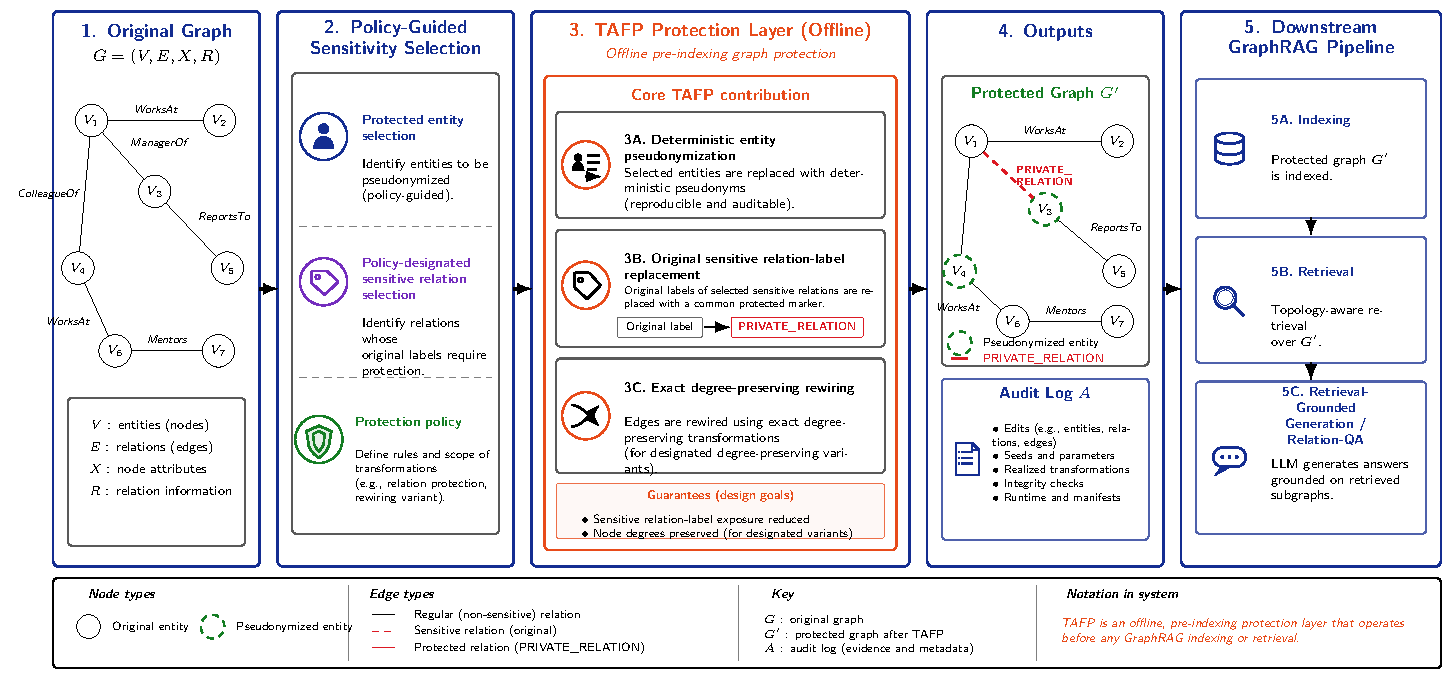
\includegraphics[width=\textwidth]{Figure_01.pdf}
\caption{TAFP-GraphRAG offline protection and downstream GraphRAG workflow. The original attributed graph first passes through a policy-guided selection stage that identifies entities selected for pseudonymization and relations designated as sensitive. The offline TAFP layer then pseudonymizes the selected entities deterministically, conceals the original labels of designated sensitive relations, and applies rewiring that preserves every node degree exactly in the designated degree-preserving variants. The protected graph is subsequently used for indexing, retrieval, and retrieval-grounded relation question answering. The transformation-audit record remains with the graph owner and is not supplied as downstream context.}
\label{fig:1}
\end{figure}

\subsection{Protection and Utility Objectives}

The framework is evaluated against five distinct objectives. First, the exposed labels of policy-designated sensitive relations should be concealed. Second, non-sensitive relation semantics should be retained when the policy permits. Third, designated degree-preserving variants should retain the exact degree of every node. Fourth, the protected graph should retain sufficient path, neighborhood, and relation evidence for the predefined retrieval and relation-question-answering tasks. Fifth, transformation behavior should remain reproducible and auditable through fixed seeds, integrity checks, run-level records, exact executable-source identities, and hash-verified artifacts.

These objectives are intentionally separate. Exact degree preservation is a deterministic structural invariant, not a privacy guarantee. Retaining endpoint reachability does not imply preservation of the original path, relation semantics, community structure, or other higher-order topology. Likewise, concealment of an original sensitive relation label does not imply that original-edge existence, policy membership, or the relation class cannot be inferred through another observation surface.

TAFP-GraphRAG is therefore assessed as an empirical, policy-conditioned protection mechanism. It does not provide differential privacy or local differential privacy, and it does not claim complete anonymization, raw-text confidentiality, document-membership privacy, edge privacy, topology privacy, or universal protection against all attackers.

\subsection{Adversary Model and Evaluation Scope}

The adversary is protocol specific. Depending on the evaluation, the adversary may observe the protected graph, protected node labels or pseudonyms, permitted node types, protected relation labels, transformed connectivity, and protocol-defined labeled training examples. Explicit sensitivity indicators, sensitivity scores, raw audit records, and original relation labels are excluded unless a protocol explicitly uses them as ground truth for evaluation.

The evaluation separates six primary exposure channels: direct recovery of original relation labels; inference that a node pair was connected in the original graph; structure-only relation inference; spectral-embedding relation inference; released-view attribute-aware GCN-GAE relation inference; and disclosure of original sensitive relations through retrieval-grounded model outputs. A separate sensitivity-marker audit tests whether released protected-label patterns reveal membership in the supplied sensitive-policy set. Policy-misclassification experiments evaluate dependence on the supplied policy rather than a new adversarial observation channel.

The released-view and locked end-to-end protocols exclude raw source text. A distinct controlled seed-42 model-facing protocol includes node-text fields truncated to 180 characters and is used only to test whether a generator transmits a relation token already exposed in the transformed context. That controlled context must not be conflated with either the released-view attacker or the locked end-to-end protocol.

The study evaluates fixed, predefined attacks and query sets. Adaptive multi-turn extraction, unrestricted free-form graph reconstruction, coordination across multiple releases, continual-update attacks, and complete subgraph reconstruction are outside the evaluated scope. The resulting claims are therefore tied to the specified datasets, policies, models, released attributes, attack features, and observation surfaces.

\begin{figure}[p]
\centering
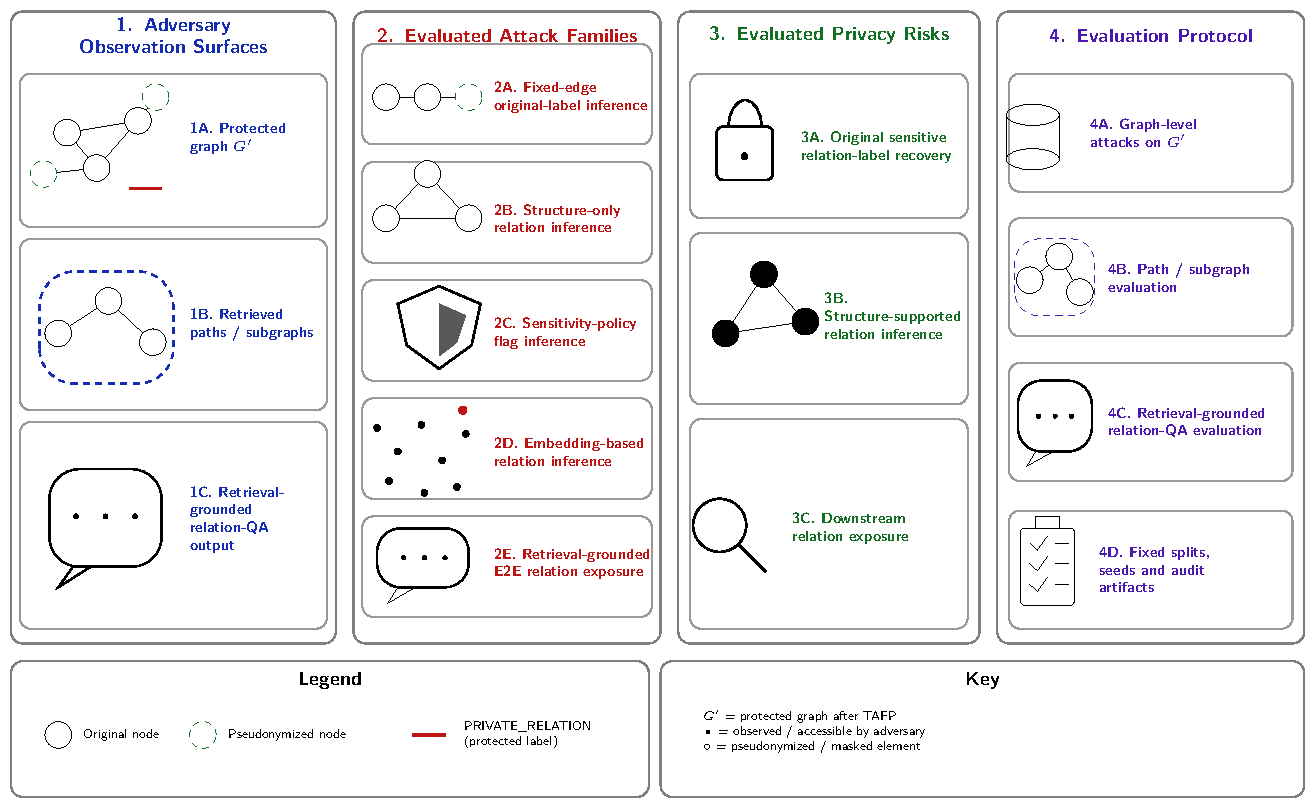
\includegraphics[width=\textwidth]{Figure_02.pdf}
\caption{Threat model and attack-evaluation scope. The adversary is evaluated across three observation surfaces: the released protected graph, retrieved path or subgraph context, and retrieval-grounded relation-question-answering output. The primary analyses cover direct original-sensitive-label exposure, original-edge-existence inference, structure-only and released-view relation inference, embedding-based relation inference, and end-to-end relation exposure. A separate marker-leakage audit tests whether released protected-label patterns reveal policy membership. The explicit internal sensitivity-policy flag and transformation-audit records are not part of the released view.}
\label{fig:2}
\end{figure}

\section{TAFP-GraphRAG Protection Framework}
Building on the graph definition in Eq. (1) and the transformation interface in Eq. (2), TAFP-GraphRAG is implemented as an offline, policy-guided transformation applied before GraphRAG indexing and retrieval.

The implementation decomposes the transformation into four ordered operations:

\begin{equation}T_{\theta,z}=W_T^{\rho_T}\circ W_R^{\rho_R}\circ S_E\circ P_V.\end{equation}
Here, P\_V pseudonymizes policy-selected entity labels, S\_E conceals the exposed labels of policy-designated sensitive relations, W\_R applies relation-level rewiring at rate $\rho$\_R, and W\_T applies topology-level rewiring at rate $\rho$\_T.

The composition is read from right to left; relation-semantic concealment therefore precedes both structural phases.

The transformation returns the protected graph G$'$ and an implementation-level transformation-audit record A.

In the designated degree-preserving variants, the structural operations satisfy the first-order invariant

\begin{equation}d_{G'}(v)=d_G(v),\ \forall v\in V.\end{equation}
This invariant applies to node degrees only; it does not imply preservation of connected components, paths, clustering, motifs, communities, spectral properties, or retrieval neighborhoods.

\subsection{Policy-Guided Selection and Deterministic Pseudonymization}
A node is eligible for policy-guided pseudonymization when its PII indicator is true or its semantic-sensitivity value is at least the policy threshold.

The implementation ranks eligible nodes by the score 2 $\times$ PII + sensitivity, where the Boolean PII indicator is interpreted numerically.

Equal scores are ordered deterministically by a hash-derived tie value computed from the node identifier and protection seed z.

The default node-sensitivity threshold is 0.45 and the default entity-selection rate is 0.75.

The selected-node target is obtained by applying Python's built-in rounding to the eligible-candidate count multiplied by the selection rate; for a positive rate and a non-empty candidate set, the target is raised to at least one and capped at the candidate count.

Each selected entity receives an exposed alias of the form \path{ENT_<LEVEL>_<HASH>}.

The implemented level function assigns HIGH when PII is true or sensitivity is at least 0.70, MED when PII is false and sensitivity is at least 0.45, and LOW otherwise.

The suffix is the first eight hexadecimal characters of \path{md5(f"{node}-{z}")}.

This MD5-derived suffix is used only to obtain deterministic experimental aliases; it is not encryption, keyed hashing, or a claim of irreversible anonymization.

The implementation contains no separate alias-collision detection or collision-resolution mechanism, and no global alias-uniqueness guarantee is made.

\subsection{Relation-Semantic Concealment and Structural Transformation}
The relation policy designates sensitive edges using an explicit internal indicator and/or a relation-sensitivity score, with a default score threshold of 0.45.

These values are operational policy inputs rather than calibrated probabilities or differential-privacy parameters.

Before structural rewiring, the exposed protected relation label of every policy-designated sensitive edge is replaced by PRIVATE\_RELATION.

This replacement conceals the original relation type through the released label field, but the marker can reveal latent membership in the policy-protected set; original-label concealment and marker-membership concealment are therefore evaluated as distinct objectives.

The relation phase operates on the current edges that satisfy the internal sensitivity rule, whereas the topology phase operates on the complete current edge set after the relation phase.

For every accepted double-edge switch, the current attribute dictionary of the first source edge is copied to the first inserted edge, and the current attribute dictionary of the second source edge is copied to the second inserted edge.

During relation-level rewiring, each copied dictionary is sanitized before insertion by setting relation\_type and protected\_relation\_type to PRIVATE\_RELATION, sensitive to 0, and relation\_sensitivity to 0.0.

During topology-level rewiring, the corresponding current source-edge dictionaries are transferred unchanged, with no additional topology-phase sanitization.

The implementation therefore uses an order-specific transfer rule; source attributes are neither randomly assigned to inserted edges nor merged.

\subsection{Exact Per-Node Degree-Preserving Rewiring}
For a phase with m candidate edges and rate $\rho$, the target rewired-edge count is zero when m < 2 or $\rho$ $\leq$ 0.

Otherwise, the implementation computes int(round(m $\times$ $\rho$)), raises the result to at least two, caps it at m, and subtracts one when the capped value is odd.

The resulting value is the target number of rewired edges, not the target number of accepted switches, because each accepted switch rewires two edges.

The proposal limit is max(2000, 300n), where n is the target rewired-edge count.

If this limit is exhausted before n edges are rewired, execution completes without an exception and returns the target and realized counts separately; convergence to the target is not guaranteed.

Given source edges \{u,v\} and \{x,y\}, a proposal is considered only when both source edges still exist and the four endpoints are distinct.

A proposed reconnection is accepted only when it creates no self-loop, the two inserted edges are distinct, and neither inserted edge already exists.

Each accepted switch removes one incident edge and adds one incident edge for every participating endpoint.

Consequently, variants composed of these accepted switches preserve every node's degree exactly, as stated in Eq. (4).

This guarantee is restricted to the designated degree-preserving variants and is not extended to higher-order graph properties.

\begin{figure}[p]
\centering
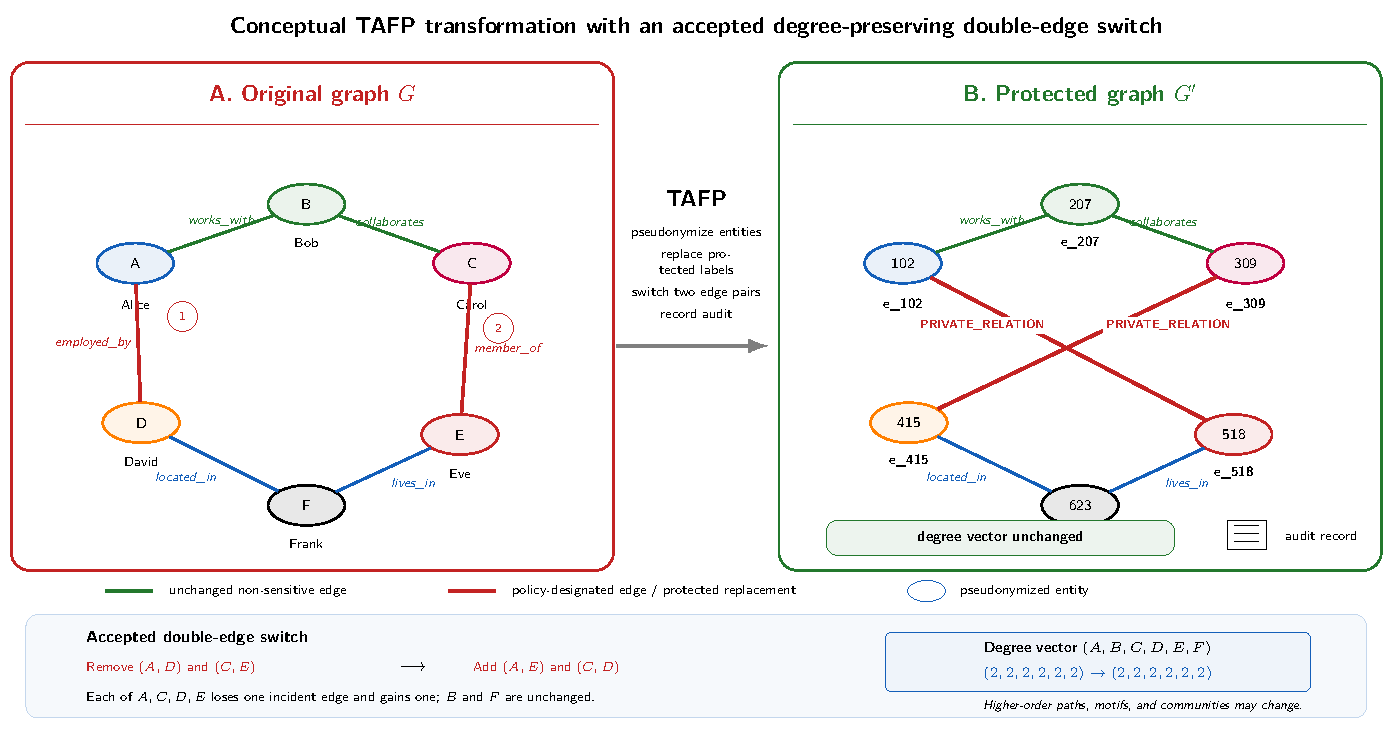
\includegraphics[width=\textwidth]{Figure_03.pdf}
\caption{Conceptual relation-phase example of an accepted degree-preserving double-edge switch in TAFP-GraphRAG. The original sensitive edges (A,D) and (C,E) are removed and replaced by (A,E) and (C,D). In this illustration, both source relations have already been assigned the protected label PRIVATE\_RELATION; therefore, both inserted edges are released with that protected label. Because each of A, C, D, and E loses one incident edge and gains one, every node degree remains unchanged. The example illustrates the relation-focused case and the degree invariant only; higher-order paths, motifs, and communities may change.}
\label{fig:3}
\end{figure}
\subsection{Auditable Execution and Operating-Point Selection}
The in-application \path{protection_audit} record stores implementation-level summaries rather than a complete event-by-event transformation history.

Its verified fields are \path{sensitive_node_candidates}, \path{masked_nodes}, \path{entity_mask_rate}, \path{sensitive_edges}, \path{relation_rewired_edges}, \path{relation_target_edges}, \path{topology_rewired_edges}, \path{topology_target_edges}, \path{degree_changed_nodes}, and \path{degree_preserved_exactly}.

The record is not described as containing complete removed-edge lists, added-edge lists, or pseudonymized-node lists.

Protection seeds, runtime measurements, and artifact hashes are maintained in separate run-level tables and hash-verified manifests rather than being assumed to reside inside \path{protection_audit}.

The study's default parameter values are pre-specified operating points and are examined through the reported ablations; they were not selected through held-out deployment calibration.

For deployment, an operator may define acceptable concealment, non-sensitive retention, and structural requirements on held-out policy-calibration data, select the least disruptive configuration that satisfies those requirements, and confirm it on a separate audit set.

This is an empirical configuration procedure, not formal privacy accounting.

\subsubsection*{Algorithm 1. Policy-guided TAFP-GraphRAG transformation}
\noindent\textbf{Input:} original simple undirected attributed graph G; protection policy $\pi$; transformation parameters $\theta$, including the entity-selection rate, $\rho$\_R, and $\rho$\_T; protection seed z.\par
\noindent\textbf{Output:} protected graph G$'$; implementation-level transformation-audit record A.\par
1. Copy G to G$'$ and initialize A.

2. Identify the policy-eligible entity candidates in G$'$.

3. Rank candidates by 2 $\times$ PII + sensitivity; resolve equal scores deterministically from the node identifier and z.

4. Compute the entity-selection target using Python rounding, the positive-rate minimum of one, and the candidate-count cap.

5. For each selected entity, assign HIGH, MED, or LOW and replace its exposed label with \path{ENT_<LEVEL>_<HASH>}.

6. Replace the exposed labels of policy-designated sensitive relations with PRIVATE\_RELATION.

7. Relation phase: form the current sensitive-edge candidate set; compute n using the verified rounding, minimum, cap, and even-parity rules; set the proposal limit to max(2000, 300n); apply the switch-acceptance checks; copy first-source attributes to the first inserted edge and second-source attributes to the second; sanitize the copied relation attributes before insertion; increase the realized rewired-edge count by two for each accepted switch.

8. Topology phase: use the complete current edge set; compute the target and proposal limit with $\rho$\_T; apply the same acceptance checks; transfer corresponding current source-edge attributes unchanged; increase the realized rewired-edge count by two for each accepted switch.

9. Compare the degree of every node in G$'$ with its degree in G.

10. Record the verified implementation-level audit summaries in A.

11. Return G$'$ and A.

\section{Experimental Design and Evaluation Methodology}
\subsection{Dataset-Derived Graphs and Fixed Evaluation Protocol}
The evaluation used five dataset-derived graphs: AGNews \cite{ref44_zhang_2015}, CNN/DailyMail \cite{ref28_nallapati_2016}, IMDB \cite{ref23_maas_2011}, PubMed \cite{ref06_cohan_2018}, and SynthPII, which was generated specifically for this study. AGNews was based on a four-class news-classification corpus, IMDB on the Large Movie Review Dataset, CNN/DailyMail on article--summary pairs, and PubMed on biomedical articles and abstracts from a long-document summarization collection. SynthPII was constructed to represent synthetic personally identifiable entities and sensitive workflow relations.

Dataset-specific adapters converted each source into a simple undirected attributed NetworkX graph. Depending on the dataset, nodes represented documents, summaries, reviews, topics, entities, biomedical concepts, or synthetic organizational records. Edges represented typed semantic relationships between node pairs. Self-loops and duplicate undirected edges were excluded during graph construction.

The resulting graphs contained 2,614 nodes and 6,542 edges for AGNews; 4,953 nodes and 15,248 edges for CNN/DailyMail; 3,119 nodes and 8,102 edges for IMDB; 1,070 nodes and 4,254 edges for PubMed; and 800 nodes and 2,400 edges for SynthPII.

Graph-construction rules, node and edge ordering, evaluation candidates, and query definitions were held constant across all protection variants and protection seeds. The structural-utility protocol comprised 2,208 fixed paths and 750 source--hop contexts defined before protection. The same source nodes, target nodes, original paths, and hop radii were reused across conditions. Table 1 reports the dataset and fixed-protocol characteristics.

\begingroup
\scriptsize
\setlength{\tabcolsep}{1.5pt}
\begin{longtable}{|L{0.19\linewidth}|C{0.13\linewidth}|C{0.13\linewidth}|C{0.17\linewidth}|C{0.22\linewidth}|}
\caption{Dataset and experimental-protocol characteristics. Fixed paths and source-hop contexts were defined before protection and reused across all variants and seeds.}\label{tab:1}\\
\hline
\makecell[bc]{\fontsize{5.2}{5.8}\selectfont\bfseries Dataset} & \makecell[bc]{\fontsize{5.2}{5.8}\selectfont\bfseries Nodes} & \makecell[bc]{\fontsize{5.2}{5.8}\selectfont\bfseries Edges} & \makecell[bc]{\fontsize{5.2}{5.8}\selectfont\bfseries Fixed paths} & \makecell[bc]{\fontsize{5.2}{5.8}\selectfont\bfseries Source-hop\\contexts} \\ \hline
\endfirsthead
\hline
\makecell[bc]{\fontsize{5.2}{5.8}\selectfont\bfseries Dataset} & \makecell[bc]{\fontsize{5.2}{5.8}\selectfont\bfseries Nodes} & \makecell[bc]{\fontsize{5.2}{5.8}\selectfont\bfseries Edges} & \makecell[bc]{\fontsize{5.2}{5.8}\selectfont\bfseries Fixed paths} & \makecell[bc]{\fontsize{5.2}{5.8}\selectfont\bfseries Source-hop\\contexts} \\ \hline
\endhead
AGNews & 2,614 & 6,542 & 438 & 150 \\ \hline
CNN\_DM & 4,953 & 15,248 & 448 & 150 \\ \hline
IMDB & 3,119 & 8,102 & 436 & 150 \\ \hline
PubMed & 1,070 & 4,254 & 442 & 150 \\ \hline
SynthPII & 800 & 2,400 & 444 & 150 \\ \hline
\end{longtable}
\endgroup
\subsection{Sensitivity Policies and Experimental Operating Points}

Each dataset-derived graph contains node- and edge-level policy attributes used to define the experimental protection scope. A node is eligible for entity pseudonymization when its PII indicator is true or its sensitivity score is at least 0.45. Eligible nodes are ranked by $2\times\mathrm{PII}+\mathrm{sensitivity}$, with deterministic seed-dependent tie ordering. The default entity-selection rate is 0.75. The selected-node target is obtained by applying the implementation's integer-rounding and bounding rules to 0.75 times the eligible-candidate count; it is not asserted to equal exactly 75\% in every graph.

An edge is policy sensitive when its internal sensitivity indicator is true or its relation-sensitivity score is at least 0.45. The default relation-level rewiring rate is 0.12 and the default topology-level rewiring rate is 0.08. These values are pre-specified experimental operating points rather than calibrated probabilities, privacy budgets, or formal risk scores.

In the final loaded graphs, the numbers and proportions of policy-sensitive edges were 3,552 of 6,542 (54.30\%) for AGNews, 13,996 of 15,248 (91.79\%) for CNN/DailyMail, 5,680 of 8,102 (70.11\%) for IMDB, 4,101 of 4,254 (96.40\%) for PubMed, and 2,207 of 2,400 (91.96\%) for SynthPII. These graph-level prevalences describe the original proxy policies used in the primary matrix.

A separate minority-sensitive ablation evaluated target prevalences of 5\%, 10\%, 20\%, and 30\%. For each dataset, the node file was copied unchanged, edge-row structure and relation information were retained, the original sensitivity indicator was copied to \nolinkurl{original_sensitive}, and the active \nolinkurl{sensitive} field was reset and reassigned deterministically. Selected rows were drawn only from the original policy-positive candidate set using policy seed 20260621. The ablation therefore evaluates lower prevalence within the original policy-positive candidates; it is not a policy-misclassification experiment. Across five datasets, four prevalence levels, 15 protection seeds, and four graph conditions, the design contained 1,200 conditions. The PubMed source-row targets were 216, 433, 865, and 1,298 for the four prevalence levels.

Hyperparameter sensitivity was evaluated one factor at a time. Entity-selection rates were 0.50, 0.75, and 1.00; relation-level rewiring rates were 0.06, 0.12, and 0.18; and topology-level rewiring rates were 0.04, 0.08, and 0.12. All non-varied parameters remained at their default values, and the same 15 protection seeds were used for every setting.

\subsection{Protection Variants and Matched Controls}

The primary experimental matrix used 15 protection seeds: 1, 7, 21, 42, 99, 123, 202, 303, 404, 505, 606, 707, 808, 909, and 1001. Five datasets and seven primary variants produced 525 graph conditions.

\nolinkurl{baseline} applied no pseudonymization, relation-label concealment, rewiring, or deletion. \nolinkurl{relation_only} replaced sensitive relation labels with \nolinkurl{PRIVATE_RELATION} and applied relation-level degree-preserving rewiring to sensitive-edge candidates, without entity pseudonymization or topology-level rewiring. \nolinkurl{topology_only} applied topology-level degree-preserving rewiring over the complete current edge set, without entity pseudonymization or systematic sensitive-label replacement. \nolinkurl{full} combined entity pseudonymization, sensitive-label concealment, relation-level rewiring, and topology-level rewiring.

Three controls separated sensitivity guidance from transformation quantity and structural preservation. \nolinkurl{random_relation_budget} selected from the complete edge set the same number of edges as the policy-sensitive count and applied the same relation target rules as \nolinkurl{relation_only}. \nolinkurl{random_edge_dropout} removed an even number of uniformly sampled edges without adding replacements; it is an intentionally non-degree-preserving deletion reference, not a matched sensitivity-guidance control. \nolinkurl{random_full_budget} randomly selected the same entity target count and edge budget as \nolinkurl{full} and used the same relation and topology rates, while removing policy guidance.

The pre-specified semantic-selectivity comparisons were \nolinkurl{relation_only} versus \nolinkurl{random_relation_budget} and \nolinkurl{full} versus \nolinkurl{random_full_budget}. These comparisons isolate whether sensitivity guidance changes which relation semantics are concealed and retained when transformation quantity is matched.

A separate sensitivity-blind 2K control, internally named \nolinkurl{dk2_full_budget}, used the same entity, relation, and topology targets as the full-budget conditions. It preserved exact per-node degree and the complete undirected joint-degree distribution. The 2K experiment added 75 unique transformations across five datasets and 15 seeds. The three-way full, \nolinkurl{random_full_budget}, and 2K analysis contained 225 condition records; the full and random-full records were reused from the primary matrix rather than regenerated.

The controls answer different questions. Random edge dropout measures structural deletion, the matched random controls isolate policy guidance at comparable transformation budgets, and the 2K control tests whether stronger degree-distribution preservation alone reproduces the selective semantic behavior of TAFP-GraphRAG. None is treated as a universal lower or upper bound on privacy or utility.

\subsection{Security and Privacy Evaluation Protocols}
Protection was evaluated under distinct adversarial observation surfaces rather than being reduced to a single privacy score. The protocols separately examined inference of original edge existence, recovery of original relation types after explicit labels had been excluded, inference of supplied-policy membership from released protection markers, robustness to incorrect sensitivity assignments, and relation inference from learned graph representations.

The fixed-edge protocol measured residual evidence that a node pair had been connected in the original graph. Sensitive and non-sensitive positive edges were evaluated as separate target groups. For each positive edge, a unique negative pair absent from the original graph was generated and matched to the positive pair by endpoint-degree classes. Across five datasets, 15 protection seeds, seven primary variants, and two target groups, the protocol contained 1,050 condition summaries and 210,000 candidate-level records. Reported outcomes were local structural AUC, hybrid edge-inference AUC, positive-edge retention, original relation-label recovery, conditional relation recovery among retained edges, and the negative false-edge rate.

The structure-only relation-inference protocol tested whether an edge's original relation type could be predicted from local topology after explicit relation labels and released node attributes had been excluded. PubMed and SynthPII were evaluated under ten stratified train-test partitions, 15 protection seeds, and seven primary variants, yielding 2,100 attack conditions. Endpoint-pair features comprised endpoint-degree summaries, common-neighbor measures, Jaccard and resource-allocation scores, endpoint clustering statistics, shortest-path distance after removal of the target edge, and an indicator for disconnected endpoint pairs. Entity types and neighboring released relation-label distributions were excluded. Feature dictionaries were vectorized, scaled without mean centering, and classified using L2-regularized multinomial logistic regression. Macro-F1 was the primary outcome and balanced accuracy the secondary outcome.

A separate sensitivity-marker protocol tested whether released protected-label patterns disclosed whether an original edge belonged to the supplied sensitive-policy set. Before transformation, each original edge was assigned provenance fields containing its original endpoint pair, original relation label, original policy-sensitivity class, and a deterministic cover-set score. Five datasets and 15 protection seeds were evaluated under seven release modes: the default private marker, relation-label omission, and shared coarse-cover settings applied to 10\%, 25\%, 50\%, 75\%, or 100\% of non-sensitive relations, yielding 525 conditions. The protocol separately measured provenance-level policy-membership AUC, marker precision, provenance-level sensitive-relation concealment, endpoint-conditioned concealment, global non-sensitive semantic retention, original-edge retention, retained-endpoint collisions, and exact degree preservation. Comparisons between each shared-cover mode and the default private marker used paired exact sign-flip tests, 20,000-replicate bootstrap confidence intervals for mean differences, and Holm adjustment within each tested metric.

Sensitivity-policy quality was evaluated through a separate misclassification-robustness protocol. For every dataset and protection seed, the clean oracle policy was perturbed using deterministic edge-level scores. False-negative scenarios removed supplied-policy labels only from oracle-sensitive edges, false-positive scenarios added labels only to oracle-non-sensitive edges, and symmetric scenarios allowed both error types. Error rates of 5\%, 10\%, and 20\% were defined from common deterministic scores, making the perturbation sets nested within each error family. Five datasets, 15 protection seeds, and ten policy scenarios produced 750 conditions. Supplied-policy fidelity measures were reported separately from oracle-grounded concealment and preservation measures so that faithful execution of an incorrect supplied policy was not interpreted as protection under the original policy. The protocol also audited exact degree and edge-count preservation. Each noisy-policy condition was compared with the clean-policy condition using paired exact sign-flip tests, 20,000-replicate bootstrap confidence intervals, and Holm adjustment within each metric.

Embedding-based relation inference was evaluated from deterministic 16-dimensional spectral node representations. For each protected graph, the adjacency matrix was symmetrically normalized as D$^{-}$$^{1}$/$^{2}$ A D$^{-}$$^{1}$/$^{2}$. The largest 17 eigenvectors were computed, the leading eigenvector was excluded, and the remaining 16 dimensions were row normalized. For each evaluated endpoint pair, the attack representation concatenated the absolute embedding difference, Hadamard product, vector sum, dot product, and Euclidean distance; no relation label was included as an input feature. PubMed and SynthPII were evaluated over 15 protection seeds, ten edge-disjoint split seeds, five graph variants, and two attack models, yielding 3,000 model evaluations. The first attacker used standardized multinomial logistic regression with balanced class weights. The second used standardized features, deterministic class-balanced resampling of the training set, and a multilayer perceptron with hidden layers of 64 and 32 units. Macro-F1, balanced accuracy, and accuracy were recorded, together with degree-preservation, edge-count, convergence, and split-integrity audits.

The spectral results were analyzed with a locked paired post-analysis. The 3,000-row source file was hash-verified before and after analysis. For each dataset, attack model, metric, and predefined variant comparison, observations were paired by protection seed and split seed. Statistical inference used a Wilcoxon signed-rank test on protection-seed cluster means, deterministic 5,000-replicate hierarchical-bootstrap confidence intervals that resampled protection-seed clusters and then split-level observations within clusters, and Holm adjustment both globally and within metric. The post-analysis generated 20 summary rows, 48 paired-test rows across Macro-F1, balanced accuracy, and accuracy, and a 16-row Macro-F1 subset.

For the broadest released-view attack, an explicit \path{TAFP_RELEASE_VIEW_V1} projection was applied before model training. Node keys were replaced with protected labels or pseudonyms; only \path{entity_type} was retained on nodes and the released protected relation type on edges. Raw text, original node and relation labels, sensitivity indicators and scores, and audit metadata were removed. A two-layer GCN graph autoencoder with 64 hidden units, a 32-dimensional output, and 160 training epochs generated node representations. Endpoint-pair classification used a class-balanced (64, 32) multilayer perceptron under three feature modes: topology only; topology plus entity type; and topology plus entity type together with target-edge-excluded distributions of neighboring released protected relation labels.

The released-view GCN-GAE protocol evaluated PubMed and SynthPII under the baseline, full TAFP-GraphRAG, and \nolinkurl{random_full_budget} conditions across 15 protection seeds, ten locked split seeds, and three feature modes, yielding 2,700 model evaluations. GCN representations were learned transductively from the complete released topology, so target-edge existence remained observable. Relation-classifier training and test edges were disjoint, and the target edge's own protected relation label was excluded from all pair-specific released-attribute features. Macro-F1, balanced accuracy, and accuracy were reported.

\subsection{Structural and Retrieval-Grounded Utility Evaluation}
Structural retrieval support was evaluated using query definitions fixed on each original graph before protection. A deterministic protocol seed of 20260618 was used to order candidate nodes. For each dataset, 50 source nodes were selected, and up to three targets were sampled at each original shortest-path distance of one, two, and three hops. The resulting protocol contained 2,208 fixed source--target paths and 750 unique source--hop contexts across the five datasets. The same paths, sources, targets, and hop radii were reused for all 15 protection seeds and seven primary variants, yielding 231,840 path-level records and 78,750 relevant-subgraph records.

For each fixed path, query-support edge retention was defined as the fraction of original path edges that remained between the same endpoints after transformation. The protocol also recorded whether the complete original path was preserved, whether the endpoints remained reachable, whether they remained reachable within the original hop count or within three hops, the protected shortest-path length, and path stretch relative to the original hop count. Original-path records additionally measured retained sensitive- and non-sensitive-edge rates, concealment of original sensitive-relation labels, and retention of original non-sensitive relation semantics.

Relevant-subgraph utility was evaluated separately for every fixed source and hop radius. The original context contained nodes reachable from the source at distances from one through the specified hop radius and the edges induced by those nodes together with the source. The corresponding context was reconstructed on each transformed graph. Original and transformed contexts were compared using relevant-node recall, precision, and Jaccard similarity, together with relevant-edge recall and Jaccard similarity. These measures quantify structural support for the fixed retrieval tasks; they do not by themselves establish generated-answer correctness, completeness, or semantic equivalence.

A controlled model-facing relation-token protocol evaluated whether an instruction-tuned generator propagated the relation label already exposed in transformed graph context. The protocol contained 200 fixed endpoint pairs, with 40 queries from each dataset, and evaluated baseline, \nolinkurl{relation_only}, full, \nolinkurl{random_relation_budget}, and \nolinkurl{random_full_budget}. The seed-42 generation run used Qwen/Qwen2.5-3B-Instruct with deterministic decoding (do\_sample=False) and at most 12 generated tokens, producing 1,000 outputs. Its controlled context included protected node labels, entity types, node-text fields truncated to 180 characters, the exposed source--target relation, and deterministic local-edge evidence. The prompt required exactly one label from a query-specific allowed-label list. This protocol isolates transmission of an already exposed relation token and is distinct from both the released-view attacker and the locked retrieval-grounded end-to-end task.

The corresponding multi-seed layer evaluated the exact exposed source--target relation for the same 200 endpoint pairs across the same five variants and 15 protection seeds, producing 15,000 transformed-context records without additional language-model generation. The seed-42 records were joined to the 1,000 generated examples by query, dataset, seed, and variant so that the relation state supplied to the generator could be checked against the exact transformed graph.

The locked retrieval-grounded end-to-end protocol used 718 fixed queries selected from the pre-protection path protocol. The manifest assigned 218 queries to non-sensitive utility and 500 to sensitive disclosure; 268 queries had a one-hop budget, 251 a two-hop budget, and 199 a three-hop budget. Every query was evaluated under baseline, full, \nolinkurl{random_full_budget}, and the sensitivity-blind 2K condition for 15 protection seeds, producing 43,080 generations.

For each query-condition-seed tuple, a deterministic breadth-first search was run from the source to the target with the query's locked hop budget as the cutoff. Neighbors were expanded in lexicographic order of their string identifiers, and the first shortest path was returned. When no path was found within the cutoff, the exposed sequence was set to \path{NOT_CONNECTED}. Otherwise, path edges were serialized in source-to-target order. The completed full protocol also added at most one deterministic side edge per retrieved path node after excluding path edges and previously selected duplicates. The graph-derived prompt context contained protected node labels or pseudonyms, permitted entity types, ordered protected-relation evidence, and transformed connectivity; raw source text, sensitivity fields, and audit metadata were excluded. Qwen/Qwen2.5-3B-Instruct generated relation-label-only outputs using deterministic decoding, a fixed generation seed of 42, a maximum input length of 3,072 tokens, and at most 32 generated tokens.

Non-sensitive utility was measured using exact relation-sequence match, multiset relation-token precision, recall, and F1, retrieved-evidence recall, exact faithfulness to the retrieved relation sequence, and faithfulness-token F1. Sensitive disclosure was measured using whether any original sensitive relation token was generated, sensitive-token recall, exposure of original sensitive tokens in retrieved evidence, and response with the protected marker. The execution audit additionally checked the locked query set, expected row count, duplicate records, parse failures, query-set drift, applicable exact-degree invariants, and the 2K joint-degree invariant. Statistical pairing, multiplicity correction, audit layers, and artifact-level reproducibility controls are specified in Section 5.6.

The locked prompt contract instructed the generator to use only the numbered \texttt{RETRIEVED ORDERED PATH EVIDENCE} lines, copy the relation label between the two separators for each line in order, join labels with " > ", output exactly \path{NOT_CONNECTED} when no path was found, and return a single line without node identifiers, explanations, JSON, bullets, or code fences. The parser removed common answer prefixes and code fences, normalized arrow, pipe, and comma delimiters, mapped tokens only to the query-specific allowed relation set, and emitted \path{PARSE_ERROR} when no allowed relation could be recovered; all parse failures remained in the primary analysis.

\subsection{Statistical Analysis, Audit Layers, and Reproducibility}
Unless a protocol explicitly retained a train--test split hierarchy, inferential comparisons were paired at the protection-seed level. Values for the compared conditions were aligned by dataset and locked seed identifier; incomplete seed sets, duplicate condition rows, or missing paired values caused the corresponding audit to fail. Descriptive graph- and utility-level summaries report means and standard deviations across the 15 protection seeds defined for each protocol.

For the seed-paired graph, semantic-selectivity, controlled relation-token, global-fidelity, hyperparameter, 2K, marker-leakage, policy-error, and path/subgraph analyses, the principal inferential procedure was a two-sided exact sign-flip test applied to paired seed differences. Ninety-five-percent percentile bootstrap intervals were computed for the mean paired difference using 20,000 resamples in the controlled relation-token, global-fidelity, hyperparameter, 2K, marker-leakage, and policy-error analyses. The semantic-selectivity and structural path/subgraph analyses used 50,000 bootstrap resamples. Where generated by the protocol-specific analysis code, two-sided Wilcoxon signed-rank results, Cohen's d\_z, and matched rank-biserial effect sizes were retained as complementary diagnostics. Statistical interpretation was based on the paired difference, its interval estimate, and the multiplicity-adjusted result rather than on an unadjusted p-value alone.

Holm correction was applied within pre-specified protocol families rather than across unrelated outcomes from the entire study. The path and relevant-subgraph analyses corrected the six full-versus-comparator tests within each dataset--metric family. The primary semantic-selectivity table corrected the two matched-control comparisons within each dataset--metric family. The controlled relation-token and global-fidelity tables used protocol-wide families of 20 and 60 tests, respectively. Hyperparameter tests were corrected within the entity-selection, relation-rewiring, and topology-rewiring families, which contained 10, 40, and 40 tests. The 2K analysis used separate semantic-selectivity and structural-fidelity families containing 30 and 90 tests. The sensitivity-marker and policy-misclassification analyses corrected comparisons separately within each reported metric. A two-sided family-wise threshold of 0.05 was used after Holm adjustment.

The spectral-embedding analysis retained its nested split structure. Each comparison contained 150 paired observations from 15 protection seeds and ten split seeds. Differences were first averaged across split seeds within each protection seed for a two-sided Wilcoxon signed-rank test over 15 protection-seed clusters. The 95\% hierarchical-bootstrap interval used 5,000 replicates, resampling protection-seed clusters and then split observations within each sampled cluster. Holm-adjusted values were reported both across the complete 48-test family and within each metric. For the released-view GCN-GAE analysis, the ten split-level outcomes were averaged within each protection seed before exact sign-flip and Wilcoxon tests were applied to the 15 paired seed means; Holm correction was applied across the 36 reported comparisons.

For the end-to-end relation-question-answering analysis, query-level observations were first averaged within dataset, protection seed, variant, and task. Overall summaries then averaged dataset-level values within each protection seed. Means, standard deviations, and 95\% t-intervals were calculated across the 15 seed means. Full TAFP-GraphRAG was compared with the baseline, \nolinkurl{random_full_budget}, and 2K conditions using two-sided Wilcoxon signed-rank tests over matched seed means. Holm adjustment was applied within each scope--task--metric family across the three comparators. The primary analysis conservatively retained all 43,080 generated records, including 26 parse failures (0.06035\%); a parse-success-only analysis was produced as a sensitivity check.

Runtime was summarized by dataset and variant as the mean and standard deviation across protection seeds, both in seconds and normalized per 1,000 edges. Audit evidence was maintained at three distinct levels. First, the implementation-level \path{protection_audit} stored the numerical transformation summaries defined in Section 4. Second, run-level result and audit tables checked expected and observed row counts, duplicate and missing records, candidate and class-balance integrity, fixed query sets, determinism, degree-preservation constraints, and the 2K joint-degree invariant. Third, artifact-level manifests linked source files, result tables, supplementary materials, and analysis outputs through SHA-256 identities.

A standalone row-level \path{protection_audit} CSV was not generated; its absence is explicitly recorded and is not treated as a failed protocol audit. The fixed-edge, multisplit, structural-utility, and end-to-end execution audits were evaluated separately and passed their stated integrity checks. The archived environment record identifies Python 3.12.13, NetworkX 3.6.1, NumPy 2.4.4, pandas 3.0.2, scikit-learn 1.8.0, SciPy 1.17.1, and PyTorch 2.11.0. Exact source identities, dependency records, table-generation manifests, analysis manifests, supplementary-package manifests, and submission-package manifests were retained with cryptographic hashes.

\section{Results}
\subsection{Selective Concealment of Sensitive Relation Semantics}
Across the five evaluated datasets, the full TAFP-GraphRAG configuration concealed 0.99993--1.00000 of the original labels of policy-designated sensitive relations while retaining 0.89935--0.92193 of non-sensitive relation semantics (Table 2). Exact per-node degree preservation remained 1.00000 in every full-protection condition, and original-edge retention ranged from 0.81833 to 0.86109. The relation-only configuration achieved complete sensitive-label concealment and complete non-sensitive semantic retention on every dataset, with original-edge retention between 0.88643 and 0.93502. The reduction from perfect non-sensitive retention to approximately 0.90--0.92 therefore appeared only when topology perturbation was added to the semantic protection layer.

The perturbation-budget-matched random control preserved nearly the same fraction of original edges as the full method: the largest absolute full-minus-random difference in original-edge retention was 0.00044, and none of the five paired differences remained significant after Holm correction. Despite this matched structural budget, random full-budget perturbation concealed only 0.57838--0.96659 of sensitive labels and retained 0.03355--0.41804 of non-sensitive semantics. Full TAFP-GraphRAG was superior in all ten dataset-by-semantic-metric comparisons, with a Holm-adjusted p value of 0.000122 for each comparison (Supplementary Table S10). This separation shows that the semantic advantage was attributable to sensitivity-guided selection rather than to perturbation volume or original-edge retention alone.

The minority-sensitive ablation produced the same qualitative protection profile at 5\%, 10\%, 20\%, and 30\% policy-designated sensitive-edge prevalence (Supplementary Table S27). Across these settings, full TAFP-GraphRAG maintained mean sensitive-label concealment of 0.9995--0.9998, mean non-sensitive semantic retention of 0.9200--0.9206, original-edge retention of 0.8876--0.9149, and exact degree preservation of 1.0000. At 5\% prevalence, the random relation-budget control retained more non-sensitive semantics than the full method (0.9499 versus 0.9202) but concealed only 0.0475 of sensitive labels, compared with 0.9996 for full TAFP-GraphRAG. From 10\% through 30\% prevalence, the full method achieved both higher concealment and higher non-sensitive retention than that control, while the random full-budget control remained lower on both semantic metrics at every prevalence level. The ablation therefore supports a prevalence-stable concealment--retention profile for the sensitivity-guided method, while the magnitude of its advantage over sensitivity-blind controls remains prevalence dependent.

\begin{landscape}
\begingroup
\scriptsize
\setlength{\tabcolsep}{1.5pt}
\begin{longtable}{|L{0.08\linewidth}|L{0.16\linewidth}|C{0.16\linewidth}|C{0.16\linewidth}|C{0.14\linewidth}|C{0.17\linewidth}|}
\caption{Protection integrity and semantic selectivity across datasets and variants. Values are means $\pm$ standard deviations over 15 protection seeds. Exact degree preservation equals one only when every node retained its original degree.}\label{tab:2}\\
\hline
\makecell[bc]{\fontsize{5.2}{5.8}\selectfont\bfseries Dataset} & \makecell[bc]{\fontsize{5.2}{5.8}\selectfont\bfseries Variant} & \makecell[bc]{\fontsize{5.2}{5.8}\selectfont\bfseries Original sensitive-label\\concealment} & \makecell[bc]{\fontsize{5.2}{5.8}\selectfont\bfseries Non-sensitive semantic\\retention} & \makecell[bc]{\fontsize{5.2}{5.8}\selectfont\bfseries Original-edge\\retention} & \makecell[bc]{\fontsize{5.2}{5.8}\selectfont\bfseries Exact per-node degree\\preservation} \\ \hline
\endfirsthead
\hline
\makecell[bc]{\fontsize{5.2}{5.8}\selectfont\bfseries Dataset} & \makecell[bc]{\fontsize{5.2}{5.8}\selectfont\bfseries Variant} & \makecell[bc]{\fontsize{5.2}{5.8}\selectfont\bfseries Original sensitive-label\\concealment} & \makecell[bc]{\fontsize{5.2}{5.8}\selectfont\bfseries Non-sensitive semantic\\retention} & \makecell[bc]{\fontsize{5.2}{5.8}\selectfont\bfseries Original-edge\\retention} & \makecell[bc]{\fontsize{5.2}{5.8}\selectfont\bfseries Exact per-node degree\\preservation} \\ \hline
\endhead
AGNews & baseline & 0.0000 $\pm$ 0.0000 & 1.0000 $\pm$ 0.0000 & 1.0000 $\pm$ 0.0000 & 1.0000 $\pm$ 0.0000 \\ \hline
AGNews & full & 1.0000 $\pm$ 0.0001 & 0.9196 $\pm$ 0.0026 & 0.8611 $\pm$ 0.0010 & 1.0000 $\pm$ 0.0000 \\ \hline
AGNews & \nolinkurl{random_edge_dropout} & 0.0787 $\pm$ 0.0042 & 0.9189 $\pm$ 0.0050 & 0.9202 $\pm$ 0.0000 & 0.0000 $\pm$ 0.0000 \\ \hline
AGNews & \nolinkurl{random_full_budget} & 0.5784 $\pm$ 0.0059 & 0.4180 $\pm$ 0.0069 & 0.8607 $\pm$ 0.0006 & 1.0000 $\pm$ 0.0000 \\ \hline
AGNews & \nolinkurl{random_relation_budget} & 0.5413 $\pm$ 0.0056 & 0.4551 $\pm$ 0.0066 & 0.9350 $\pm$ 0.0001 & 1.0000 $\pm$ 0.0000 \\ \hline
AGNews & \nolinkurl{relation_only} & 1.0000 $\pm$ 0.0000 & 1.0000 $\pm$ 0.0000 & 0.9350 $\pm$ 0.0001 & 1.0000 $\pm$ 0.0000 \\ \hline
AGNews & \nolinkurl{topology_only} & 0.0804 $\pm$ 0.0022 & 0.9211 $\pm$ 0.0026 & 0.9204 $\pm$ 0.0002 & 1.0000 $\pm$ 0.0000 \\ \hline
CNN\_DM & baseline & 0.0000 $\pm$ 0.0000 & 1.0000 $\pm$ 0.0000 & 1.0000 $\pm$ 0.0000 & 1.0000 $\pm$ 0.0000 \\ \hline
CNN\_DM & full & 1.0000 $\pm$ 0.0000 & 0.9171 $\pm$ 0.0093 & 0.8188 $\pm$ 0.0010 & 1.0000 $\pm$ 0.0000 \\ \hline
CNN\_DM & \nolinkurl{random_edge_dropout} & 0.0802 $\pm$ 0.0005 & 0.9221 $\pm$ 0.0051 & 0.9200 $\pm$ 0.0000 & 0.0000 $\pm$ 0.0000 \\ \hline
CNN\_DM & \nolinkurl{random_full_budget} & 0.9243 $\pm$ 0.0008 & 0.0730 $\pm$ 0.0094 & 0.8192 $\pm$ 0.0006 & 1.0000 $\pm$ 0.0000 \\ \hline
CNN\_DM & \nolinkurl{random_relation_budget} & 0.9177 $\pm$ 0.0010 & 0.0798 $\pm$ 0.0108 & 0.8900 $\pm$ 0.0001 & 1.0000 $\pm$ 0.0000 \\ \hline
CNN\_DM & \nolinkurl{relation_only} & 1.0000 $\pm$ 0.0000 & 1.0000 $\pm$ 0.0000 & 0.8900 $\pm$ 0.0001 & 1.0000 $\pm$ 0.0000 \\ \hline
CNN\_DM & \nolinkurl{topology_only} & 0.0798 $\pm$ 0.0008 & 0.9179 $\pm$ 0.0085 & 0.9201 $\pm$ 0.0001 & 1.0000 $\pm$ 0.0000 \\ \hline
IMDB & baseline & 0.0000 $\pm$ 0.0000 & 1.0000 $\pm$ 0.0000 & 1.0000 $\pm$ 0.0000 & 1.0000 $\pm$ 0.0000 \\ \hline
IMDB & full & 0.9999 $\pm$ 0.0001 & 0.9192 $\pm$ 0.0047 & 0.8429 $\pm$ 0.0012 & 1.0000 $\pm$ 0.0000 \\ \hline
IMDB & \nolinkurl{random_edge_dropout} & 0.0791 $\pm$ 0.0019 & 0.9180 $\pm$ 0.0044 & 0.9200 $\pm$ 0.0000 & 0.0000 $\pm$ 0.0000 \\ \hline
IMDB & \nolinkurl{random_full_budget} & 0.7251 $\pm$ 0.0033 & 0.2754 $\pm$ 0.0075 & 0.8429 $\pm$ 0.0009 & 1.0000 $\pm$ 0.0000 \\ \hline
IMDB & \nolinkurl{random_relation_budget} & 0.7017 $\pm$ 0.0030 & 0.3004 $\pm$ 0.0071 & 0.9159 $\pm$ 0.0001 & 1.0000 $\pm$ 0.0000 \\ \hline
IMDB & \nolinkurl{relation_only} & 1.0000 $\pm$ 0.0000 & 1.0000 $\pm$ 0.0000 & 0.9160 $\pm$ 0.0002 & 1.0000 $\pm$ 0.0000 \\ \hline
IMDB & \nolinkurl{topology_only} & 0.0804 $\pm$ 0.0020 & 0.9211 $\pm$ 0.0046 & 0.9201 $\pm$ 0.0001 & 1.0000 $\pm$ 0.0000 \\ \hline
PubMed & baseline & 0.0000 $\pm$ 0.0000 & 1.0000 $\pm$ 0.0000 & 1.0000 $\pm$ 0.0000 & 1.0000 $\pm$ 0.0000 \\ \hline
PubMed & full & 1.0000 $\pm$ 0.0000 & 0.8993 $\pm$ 0.0222 & 0.8186 $\pm$ 0.0013 & 1.0000 $\pm$ 0.0000 \\ \hline
PubMed & \nolinkurl{random_edge_dropout} & 0.0795 $\pm$ 0.0008 & 0.9081 $\pm$ 0.0224 & 0.9201 $\pm$ 0.0000 & 0.0000 $\pm$ 0.0000 \\ \hline
PubMed & \nolinkurl{random_full_budget} & 0.9666 $\pm$ 0.0011 & 0.0336 $\pm$ 0.0178 & 0.8189 $\pm$ 0.0015 & 1.0000 $\pm$ 0.0000 \\ \hline
PubMed & \nolinkurl{random_relation_budget} & 0.9640 $\pm$ 0.0007 & 0.0357 $\pm$ 0.0186 & 0.8858 $\pm$ 0.0006 & 1.0000 $\pm$ 0.0000 \\ \hline
PubMed & \nolinkurl{relation_only} & 1.0000 $\pm$ 0.0000 & 1.0000 $\pm$ 0.0000 & 0.8864 $\pm$ 0.0005 & 1.0000 $\pm$ 0.0000 \\ \hline
PubMed & \nolinkurl{topology_only} & 0.0788 $\pm$ 0.0012 & 0.9020 $\pm$ 0.0320 & 0.9209 $\pm$ 0.0003 & 1.0000 $\pm$ 0.0000 \\ \hline
SynthPII & baseline & 0.0000 $\pm$ 0.0000 & 1.0000 $\pm$ 0.0000 & 1.0000 $\pm$ 0.0000 & 1.0000 $\pm$ 0.0000 \\ \hline
SynthPII & full & 1.0000 $\pm$ 0.0000 & 0.9219 $\pm$ 0.0132 & 0.8183 $\pm$ 0.0012 & 1.0000 $\pm$ 0.0000 \\ \hline
SynthPII & \nolinkurl{random_edge_dropout} & 0.0801 $\pm$ 0.0016 & 0.9209 $\pm$ 0.0178 & 0.9200 $\pm$ 0.0000 & 0.0000 $\pm$ 0.0000 \\ \hline
SynthPII & \nolinkurl{random_full_budget} & 0.9256 $\pm$ 0.0019 & 0.0722 $\pm$ 0.0210 & 0.8188 $\pm$ 0.0016 & 1.0000 $\pm$ 0.0000 \\ \hline
SynthPII & \nolinkurl{random_relation_budget} & 0.9194 $\pm$ 0.0017 & 0.0784 $\pm$ 0.0199 & 0.8901 $\pm$ 0.0001 & 1.0000 $\pm$ 0.0000 \\ \hline
SynthPII & \nolinkurl{relation_only} & 1.0000 $\pm$ 0.0000 & 1.0000 $\pm$ 0.0000 & 0.8901 $\pm$ 0.0002 & 1.0000 $\pm$ 0.0000 \\ \hline
SynthPII & \nolinkurl{topology_only} & 0.0801 $\pm$ 0.0017 & 0.9209 $\pm$ 0.0189 & 0.9201 $\pm$ 0.0001 & 1.0000 $\pm$ 0.0000 \\ \hline
\end{longtable}
\endgroup
\end{landscape}
\begin{figure}[p]
\centering
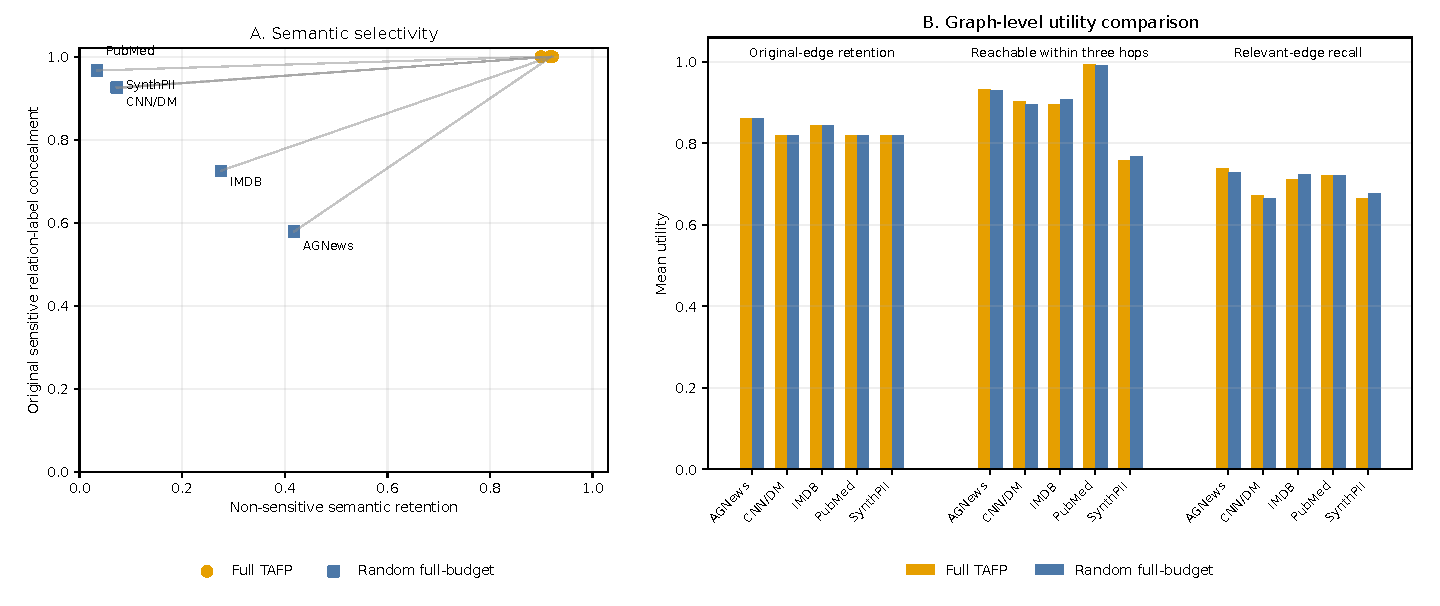
\includegraphics[width=\textwidth]{Figure_04.pdf}
\caption{Graph-level semantic selectivity and utility across the five evaluated datasets. Panel A plots mean non-sensitive semantic retention against mean original sensitive relation-label concealment for Full TAFP and the perturbation-budget-matched random full-budget control. Lines connect the two variants within each dataset. Panel B reports three manuscript-defined graph-level utility measures---original-edge retention, reachability within three hops, and relevant-edge recall---using the same two variants. Values are means over the locked protection-seed protocol; dispersion statistics remain available in the corresponding tables.}
\label{fig:4}
\end{figure}
\begin{figure}[p]
\centering
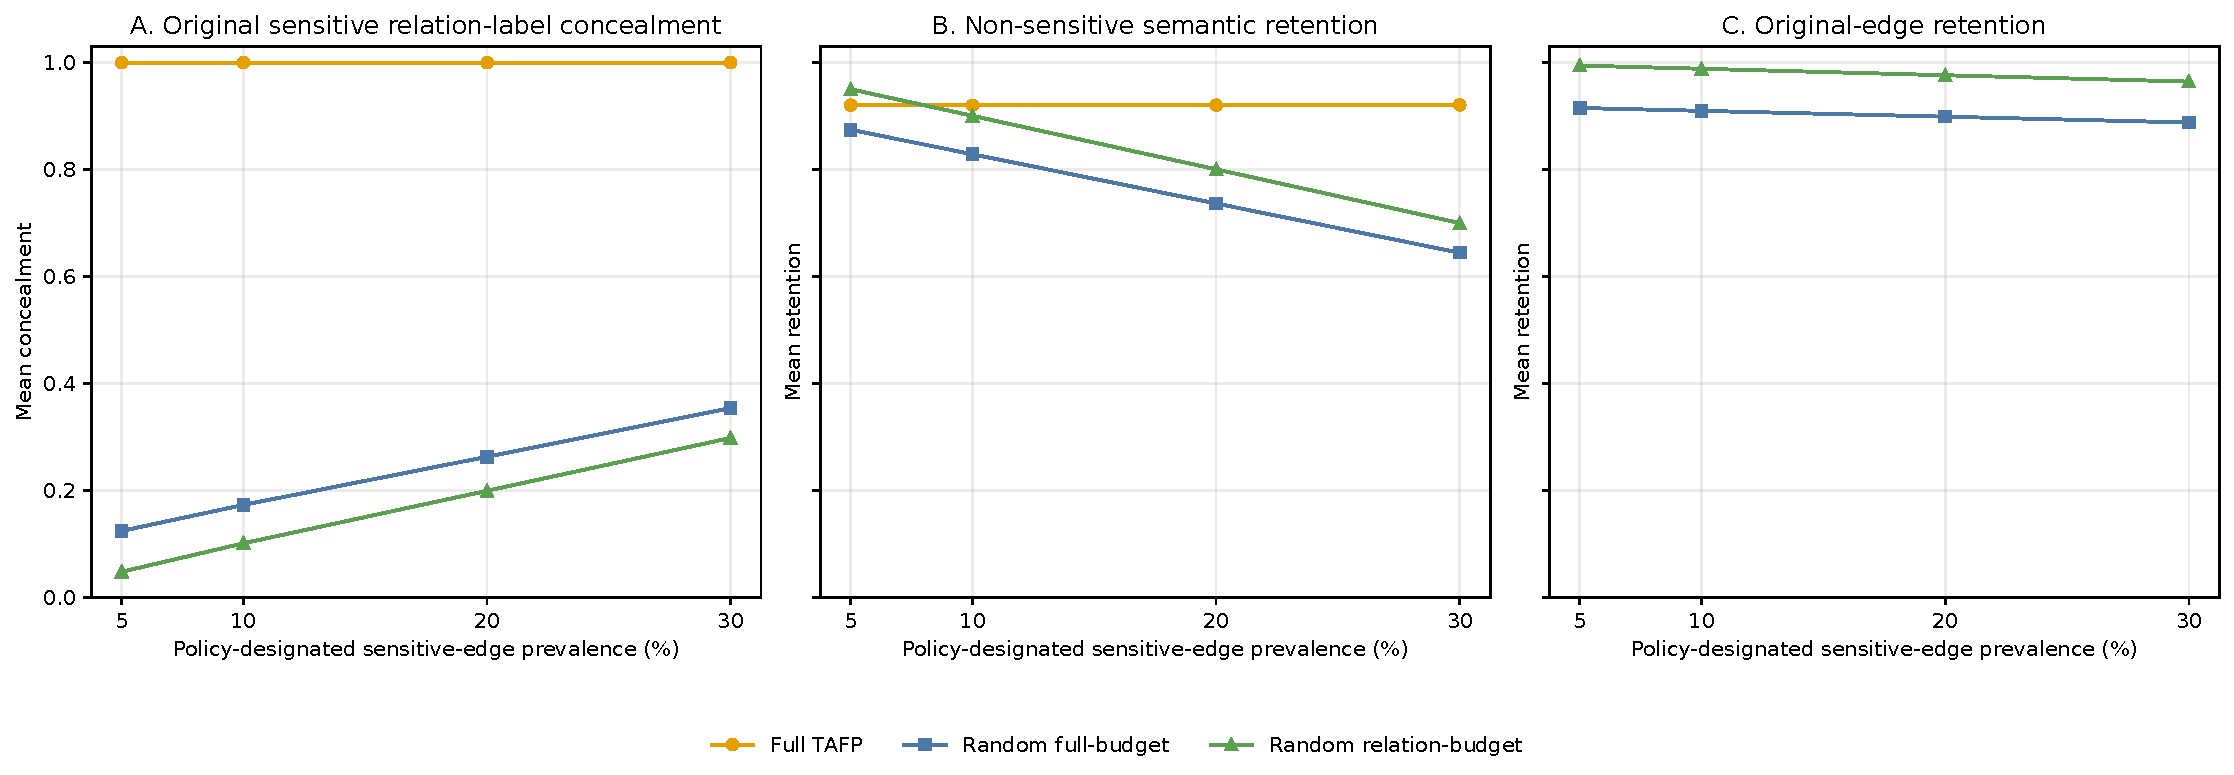
\includegraphics[width=\textwidth]{Figure_05.pdf}
\caption{Minority-sensitive policy ablation across 5\%, 10\%, 20\%, and 30\% policy-designated sensitive-edge prevalence. Panel A reports original sensitive relation-label concealment, Panel B reports non-sensitive semantic retention, and Panel C reports original-edge retention for Full TAFP and the two sensitivity-blind random controls. Points are unweighted means across the five evaluated datasets, and whiskers show the minimum-to-maximum range of the dataset-level means. Each dataset-level value summarizes the locked 15-seed protection protocol. Exact per-node degree preservation was 1.0000 for every displayed prevalence, dataset, and variant configuration.}
\label{fig:5}
\end{figure}
\subsection{Exact Degree Preservation and Structural Effects}
Across the 450 dataset--seed--variant rows corresponding to the baseline and the five degree-preserving perturbation variants, every row had zero changed-degree nodes, zero degree-sequence L1 error, and exact per-node degree preservation equal to 1. The matched random edge-dropout control behaved differently: none of its 75 rows preserved every node degree, the number of changed-degree nodes ranged from 295 to 1,690, and degree-sequence L1 error ranged from 384 to 2,440 (Supplementary Table S6). This difference was not explained by edge-retention volume. The topology-only configuration retained 0.92005--0.92089 of original edges across datasets, whereas random edge dropout retained 0.91999--0.92021; nevertheless, only the former preserved every node degree (Table 2). The full and random full-budget configurations also preserved every node degree while retaining 0.81833--0.86109 and 0.81878--0.86071 of original edges, respectively.

The 2K full-budget control imposed a stronger structural constraint. Across five datasets and 15 seeds per dataset, its exact degree-sequence rate was 1.0 and its mean joint-degree L1 error was 0 for every dataset (Supplementary Table S17). The locked summaries also reported zero component-count deviation and zero largest-component-ratio deviation. These constraints did not imply exact preservation of all higher-order structure: mean absolute clustering-coefficient deviation ranged from 0.00089 to 0.28649, and mean absolute transitivity deviation ranged from 0.00082 to 0.02185. By comparison, the full and random full-budget variants preserved individual node degrees but not the joint-degree distribution; their dataset-level mean joint-degree L1 errors ranged from 174.4 to 1,692.9 and from 160.0 to 1,695.6, respectively.

Despite the stronger 2K invariant, full TAFP-GraphRAG was better in all ten paired comparisons covering sensitive-relation concealment and non-sensitive semantic retention, with Holm-adjusted p = 0.001831 for each comparison (Supplementary Table S18). In contrast, none of the ten corresponding 2K-versus-random-full-budget comparisons was significant after Holm correction. Thus, exact individual- and joint-degree preservation constrained structural change but did not reproduce sensitivity-selective semantic protection.

\begin{landscape}
\begingroup
\scriptsize
\renewcommand{\arraystretch}{0.96}
\setlength{\tabcolsep}{1.5pt}
\begin{longtable}{|L{0.07\linewidth}|L{0.15\linewidth}|C{0.10\linewidth}|C{0.13\linewidth}|C{0.12\linewidth}|C{0.14\linewidth}|C{0.12\linewidth}|}
\caption{Transformation runtime and edit integrity. Runtime covers apply\_variant() only; values are means $\pm$ standard deviations over 15 protection seeds.}\label{tab:3}\\
\hline
\makecell[bc]{\fontsize{5.2}{5.8}\selectfont\bfseries Dataset} & \makecell[bc]{\fontsize{5.2}{5.8}\selectfont\bfseries Variant} & \makecell[bc]{\fontsize{5.2}{5.8}\selectfont\bfseries Runtime\\(s)} & \makecell[bc]{\fontsize{5.2}{5.8}\selectfont\bfseries Runtime/1000\\edges (s)} & \makecell[bc]{\fontsize{5.2}{5.8}\selectfont\bfseries Added\\edges} & \makecell[bc]{\fontsize{5.2}{5.8}\selectfont\bfseries Removed original\\edges} & \makecell[bc]{\fontsize{5.2}{5.8}\selectfont\bfseries Changed-degree\\nodes} \\ \hline
\endfirsthead
\hline
\makecell[bc]{\fontsize{5.2}{5.8}\selectfont\bfseries Dataset} & \makecell[bc]{\fontsize{5.2}{5.8}\selectfont\bfseries Variant} & \makecell[bc]{\fontsize{5.2}{5.8}\selectfont\bfseries Runtime\\(s)} & \makecell[bc]{\fontsize{5.2}{5.8}\selectfont\bfseries Runtime/1000\\edges (s)} & \makecell[bc]{\fontsize{5.2}{5.8}\selectfont\bfseries Added\\edges} & \makecell[bc]{\fontsize{5.2}{5.8}\selectfont\bfseries Removed original\\edges} & \makecell[bc]{\fontsize{5.2}{5.8}\selectfont\bfseries Changed-degree\\nodes} \\ \hline
\endhead
AGNews & baseline & 0.0580 $\pm$ 0.0348 & 0.0089 $\pm$ 0.0053 & 0.0000 $\pm$ 0.0000 & 0.0000 $\pm$ 0.0000 & 0.0000 $\pm$ 0.0000 \\ \hline
AGNews & full & 0.1354 $\pm$ 0.0452 & 0.0207 $\pm$ 0.0069 & 908.7333 $\pm$ 6.8187 & 908.7333 $\pm$ 6.8187 & 0.0000 $\pm$ 0.0000 \\ \hline
AGNews & \nolinkurl{random_edge_dropout} & 0.0911 $\pm$ 0.0560 & 0.0139 $\pm$ 0.0086 & 0.0000 $\pm$ 0.0000 & 522 $\pm$ 0.0000 & 745.8000 $\pm$ 9.7848 \\ \hline
AGNews & \nolinkurl{random_full_budget} & 0.1218 $\pm$ 0.0345 & 0.0186 $\pm$ 0.0053 & 911.2667 $\pm$ 3.6541 & 911.2667 $\pm$ 3.6541 & 0.0000 $\pm$ 0.0000 \\ \hline
AGNews & \nolinkurl{random_relation_budget} & 0.0851 $\pm$ 0.0312 & 0.0130 $\pm$ 0.0048 & 425.4667 $\pm$ 0.8338 & 425.4667 $\pm$ 0.8338 & 0.0000 $\pm$ 0.0000 \\ \hline
AGNews & \nolinkurl{relation_only} & 0.0968 $\pm$ 0.0438 & 0.0148 $\pm$ 0.0067 & 425.0667 $\pm$ 0.8837 & 425.0667 $\pm$ 0.8837 & 0.0000 $\pm$ 0.0000 \\ \hline
AGNews & \nolinkurl{topology_only} & 0.0784 $\pm$ 0.0364 & 0.0120 $\pm$ 0.0056 & 520.6000 $\pm$ 1.1832 & 520.6000 $\pm$ 1.1832 & 0.0000 $\pm$ 0.0000 \\ \hline
CNN\_DM & baseline & 0.1132 $\pm$ 0.0428 & 0.0074 $\pm$ 0.0028 & 0.0000 $\pm$ 0.0000 & 0.0000 $\pm$ 0.0000 & 0.0000 $\pm$ 0.0000 \\ \hline
CNN\_DM & full & 0.3300 $\pm$ 0.0294 & 0.0216 $\pm$ 0.0019 & 2762.3333 $\pm$ 14.4897 & 2762.3333 $\pm$ 14.4897 & 0.0000 $\pm$ 0.0000 \\ \hline
CNN\_DM & \nolinkurl{random_edge_dropout} & 0.1507 $\pm$ 0.0529 & 0.0099 $\pm$ 0.0035 & 0.0000 $\pm$ 0.0000 & 1,220 $\pm$ 0.0000 & 1663.8000 $\pm$ 16.2226 \\ \hline
CNN\_DM & \nolinkurl{random_full_budget} & 0.3363 $\pm$ 0.0397 & 0.0221 $\pm$ 0.0026 & 2756.8000 $\pm$ 9.5559 & 2756.8000 $\pm$ 9.5559 & 0.0000 $\pm$ 0.0000 \\ \hline
CNN\_DM & \nolinkurl{random_relation_budget} & 0.2315 $\pm$ 0.0594 & 0.0152 $\pm$ 0.0039 & 1677.9333 $\pm$ 1.2799 & 1677.9333 $\pm$ 1.2799 & 0.0000 $\pm$ 0.0000 \\ \hline
CNN\_DM & \nolinkurl{relation_only} & 0.2150 $\pm$ 0.0567 & 0.0141 $\pm$ 0.0037 & 1677.9333 $\pm$ 1.4376 & 1677.9333 $\pm$ 1.4376 & 0.0000 $\pm$ 0.0000 \\ \hline
CNN\_DM & \nolinkurl{topology_only} & 0.1802 $\pm$ 0.0545 & 0.0118 $\pm$ 0.0036 & 1219.0667 $\pm$ 0.9612 & 1219.0667 $\pm$ 0.9612 & 0.0000 $\pm$ 0.0000 \\ \hline
IMDB & baseline & 0.0585 $\pm$ 0.0196 & 0.0072 $\pm$ 0.0024 & 0.0000 $\pm$ 0.0000 & 0.0000 $\pm$ 0.0000 & 0.0000 $\pm$ 0.0000 \\ \hline
IMDB & full & 0.1848 $\pm$ 0.0478 & 0.0228 $\pm$ 0.0059 & 1,273 $\pm$ 9.4868 & 1,273 $\pm$ 9.4868 & 0.0000 $\pm$ 0.0000 \\ \hline
IMDB & \nolinkurl{random_edge_dropout} & 0.0831 $\pm$ 0.0389 & 0.0103 $\pm$ 0.0048 & 0.0000 $\pm$ 0.0000 & 648 $\pm$ 0.0000 & 908.5333 $\pm$ 14.5498 \\ \hline
IMDB & \nolinkurl{random_full_budget} & 0.1993 $\pm$ 0.0543 & 0.0246 $\pm$ 0.0067 & 1272.7333 $\pm$ 7.4014 & 1272.7333 $\pm$ 7.4014 & 0.0000 $\pm$ 0.0000 \\ \hline
IMDB & \nolinkurl{random_relation_budget} & 0.1482 $\pm$ 0.0594 & 0.0183 $\pm$ 0.0073 & 681.3333 $\pm$ 0.8997 & 681.3333 $\pm$ 0.8997 & 0.0000 $\pm$ 0.0000 \\ \hline
IMDB & \nolinkurl{relation_only} & 0.1149 $\pm$ 0.0438 & 0.0142 $\pm$ 0.0054 & 680.4667 $\pm$ 1.2459 & 680.4667 $\pm$ 1.2459 & 0.0000 $\pm$ 0.0000 \\ \hline
IMDB & \nolinkurl{topology_only} & 0.1153 $\pm$ 0.0508 & 0.0142 $\pm$ 0.0063 & 647.6667 $\pm$ 0.6172 & 647.6667 $\pm$ 0.6172 & 0.0000 $\pm$ 0.0000 \\ \hline
PubMed & baseline & 0.0235 $\pm$ 0.0044 & 0.0055 $\pm$ 0.0010 & 0.0000 $\pm$ 0.0000 & 0.0000 $\pm$ 0.0000 & 0.0000 $\pm$ 0.0000 \\ \hline
PubMed & full & 0.0797 $\pm$ 0.0417 & 0.0187 $\pm$ 0.0098 & 771.6667 $\pm$ 5.6904 & 771.6667 $\pm$ 5.6904 & 0.0000 $\pm$ 0.0000 \\ \hline
PubMed & \nolinkurl{random_edge_dropout} & 0.0408 $\pm$ 0.0297 & 0.0096 $\pm$ 0.0070 & 0.0000 $\pm$ 0.0000 & 340 $\pm$ 0.0000 & 343 $\pm$ 10.1489 \\ \hline
PubMed & \nolinkurl{random_full_budget} & 0.0842 $\pm$ 0.0384 & 0.0198 $\pm$ 0.0090 & 770.3333 $\pm$ 6.5320 & 770.3333 $\pm$ 6.5320 & 0.0000 $\pm$ 0.0000 \\ \hline
PubMed & \nolinkurl{random_relation_budget} & 0.0544 $\pm$ 0.0222 & 0.0128 $\pm$ 0.0052 & 485.8667 $\pm$ 2.5598 & 485.8667 $\pm$ 2.5598 & 0.0000 $\pm$ 0.0000 \\ \hline
PubMed & \nolinkurl{relation_only} & 0.0512 $\pm$ 0.0300 & 0.0120 $\pm$ 0.0071 & 483.1333 $\pm$ 2.2636 & 483.1333 $\pm$ 2.2636 & 0.0000 $\pm$ 0.0000 \\ \hline
PubMed & \nolinkurl{topology_only} & 0.0422 $\pm$ 0.0267 & 0.0099 $\pm$ 0.0063 & 336.5333 $\pm$ 1.4075 & 336.5333 $\pm$ 1.4075 & 0.0000 $\pm$ 0.0000 \\ \hline
SynthPII & baseline & 0.0148 $\pm$ 0.0033 & 0.0062 $\pm$ 0.0014 & 0.0000 $\pm$ 0.0000 & 0.0000 $\pm$ 0.0000 & 0.0000 $\pm$ 0.0000 \\ \hline
SynthPII & full & 0.0524 $\pm$ 0.0319 & 0.0218 $\pm$ 0.0133 & 436 $\pm$ 2.9761 & 436 $\pm$ 2.9761 & 0.0000 $\pm$ 0.0000 \\ \hline
SynthPII & \nolinkurl{random_edge_dropout} & 0.0180 $\pm$ 0.0035 & 0.0075 $\pm$ 0.0015 & 0.0000 $\pm$ 0.0000 & 192 $\pm$ 0.0000 & 303.7333 $\pm$ 5.8975 \\ \hline
SynthPII & \nolinkurl{random_full_budget} & 0.0355 $\pm$ 0.0079 & 0.0148 $\pm$ 0.0033 & 434.9333 $\pm$ 3.7506 & 434.9333 $\pm$ 3.7506 & 0.0000 $\pm$ 0.0000 \\ \hline
SynthPII & \nolinkurl{random_relation_budget} & 0.0300 $\pm$ 0.0050 & 0.0125 $\pm$ 0.0021 & 263.8667 $\pm$ 0.3519 & 263.8667 $\pm$ 0.3519 & 0.0000 $\pm$ 0.0000 \\ \hline
SynthPII & \nolinkurl{relation_only} & 0.0257 $\pm$ 0.0053 & 0.0107 $\pm$ 0.0022 & 263.7333 $\pm$ 0.5936 & 263.7333 $\pm$ 0.5936 & 0.0000 $\pm$ 0.0000 \\ \hline
SynthPII & \nolinkurl{topology_only} & 0.0270 $\pm$ 0.0286 & 0.0113 $\pm$ 0.0119 & 191.8667 $\pm$ 0.3519 & 191.8667 $\pm$ 0.3519 & 0.0000 $\pm$ 0.0000 \\ \hline
\end{longtable}
\endgroup
\end{landscape}
\subsection{Attack-Specific Privacy Evaluation}
The fixed-edge analysis separated concealment of the original sensitive relation label from inference of original edge existence. Under both the relation-only and full configurations, mean recovery of the original sensitive relation type was 0 on all five datasets (Table~\ref{tab:4}). This result did not eliminate structural evidence of prior connectivity. For the full configuration, local structural AUC ranged from 0.49909 to 0.86879 and hybrid edge-inference AUC from 0.90705 to 0.97351. Thus, the transformation consistently removed direct sensitive-label recovery in this protocol, while residual edge-existence inference remained dataset dependent and was substantial for several datasets.

The structure-only relation attack showed a similarly conditional pattern. On PubMed, full TAFP-GraphRAG reduced mean Macro-F1 from 0.64602 for the unprotected baseline and 0.62377 for random edge dropout to 0.61108; the one-sided Holm-adjusted p values were 0.005859 and 0.003906, respectively (Table~\ref{tab:5}). However, full was not significantly different from either perturbation-budget-matched random control. On SynthPII, full achieved Macro-F1 of 0.08635, and none of the four reported full-versus-comparator tests was significant after Holm correction. These results show that topology-only relation inference was weakened in the PubMed setting relative to unprotected and deletion-only references, but they do not establish a sensitivity-guided advantage over matched random perturbation for this attack.

Embedding-based attacks reinforced the dataset dependence. On PubMed, spectral-logistic Macro-F1 decreased from 0.72164 under the baseline to 0.57853 under full protection, and spectral-MLP Macro-F1 decreased from 0.69662 to 0.57612. Both full-versus-baseline comparisons remained significant after global Holm correction, whereas neither full-versus-random-full-budget comparison was significant (Supplementary Tables S22--S23). On SynthPII, no consistent reduction was observed: spectral-logistic Macro-F1 was slightly higher under full protection than under the baseline (0.11364 versus 0.10118; globally Holm-adjusted p = 0.015808), while the spectral-MLP comparison was not significant. Accordingly, the spectral results support a reduction in PubMed attack performance but not a general advantage across datasets or over the matched random control.

The released-view GCN-GAE stress test produced the same boundary. On PubMed, full protection reduced Macro-F1 from 0.76515 to 0.59832 with topology-only features, from 0.88081 to 0.80088 after adding entity type, and from 0.99351 to 0.85222 with the complete permitted released-attribute feature set. All nine PubMed full-versus-baseline metric comparisons were significant after exact sign-flip Holm correction. None of the nine corresponding full-versus-random-full-budget comparisons was significant. On SynthPII, none of the full-versus-baseline or full-versus-random-full-budget comparisons remained significant after correction (Supplementary Tables S28--S29). The broader learned-representation attacks therefore demonstrate reduced inference relative to the unprotected PubMed graph, while also showing that the effect cannot be attributed uniquely to sensitivity-guided selection under the matched structural budget.

The marker audit identified a separate release-policy risk. Both the default PRIVATE\_RELATION marker and relation-label omission yielded policy-membership AUC of 1.0 on every dataset. Applying the same coarse marker to 50\% of non-sensitive relations reduced AUC to 0.74597--0.75561, but also reduced non-sensitive semantic retention to 0.44401--0.47496. Applying the cover to all non-sensitive relations reduced AUC to 0.5 while reducing non-sensitive semantic retention to 0. Across all cover settings, sensitive-label concealment and exact degree preservation remained 1.0. All 50 paired AUC or retention comparisons against the default marker were significant after Holm correction (p = 0.001526). Marker privacy is therefore not obtained without a direct semantic-utility cost under the evaluated release policies.

Finally, the policy-misclassification experiment distinguished correct execution of the supplied policy from protection under the original oracle policy. Supplied-policy marker AUC and supplied-policy relation concealment remained 1.0 in every scenario, and exact edge-count and degree preservation also remained 1.0. In contrast, at a 20\% false-negative rate, oracle sensitive-relation concealment fell to 0.79979--0.80280. At a 20\% false-positive rate, oracle non-sensitive label preservation fell to 0.78791--0.80362. Under 20\% symmetric error, oracle sensitive concealment was 0.79742--0.80184 and oracle non-sensitive preservation was 0.79216--0.80656 (Supplementary Table S21). TAFP-GraphRAG therefore executed the supplied policy faithfully but did not correct errors in that policy, making policy quality an explicit operational dependency.

\begin{landscape}
\begingroup
\scriptsize
\setlength{\tabcolsep}{1.5pt}
\begin{longtable}{|L{0.07\linewidth}|L{0.15\linewidth}|C{0.12\linewidth}|C{0.12\linewidth}|C{0.12\linewidth}|C{0.15\linewidth}|C{0.12\linewidth}|}
\caption{Fixed-edge evaluation on sensitive target edges. Local structural AUC and hybrid edge AUC represent distinct attacker feature sets. Values are means $\pm$ standard deviations over 15 protection seeds.}\label{tab:4}\\
\hline
\makecell[bc]{\fontsize{5.2}{5.8}\selectfont\bfseries Dataset} & \makecell[bc]{\fontsize{5.2}{5.8}\selectfont\bfseries Variant} & \makecell[bc]{\fontsize{5.2}{5.8}\selectfont\bfseries Local structural\\AUC} & \makecell[bc]{\fontsize{5.2}{5.8}\selectfont\bfseries Hybrid edge\\AUC} & \makecell[bc]{\fontsize{5.2}{5.8}\selectfont\bfseries Positive-edge\\retention} & \makecell[bc]{\fontsize{5.2}{5.8}\selectfont\bfseries Original relation-\\label recovery} & \makecell[bc]{\fontsize{5.2}{5.8}\selectfont\bfseries Conditional\\relation recovery} \\ \hline
\endfirsthead
\hline
\makecell[bc]{\fontsize{5.2}{5.8}\selectfont\bfseries Dataset} & \makecell[bc]{\fontsize{5.2}{5.8}\selectfont\bfseries Variant} & \makecell[bc]{\fontsize{5.2}{5.8}\selectfont\bfseries Local structural\\AUC} & \makecell[bc]{\fontsize{5.2}{5.8}\selectfont\bfseries Hybrid edge\\AUC} & \makecell[bc]{\fontsize{5.2}{5.8}\selectfont\bfseries Positive-edge\\retention} & \makecell[bc]{\fontsize{5.2}{5.8}\selectfont\bfseries Original relation-\\label recovery} & \makecell[bc]{\fontsize{5.2}{5.8}\selectfont\bfseries Conditional\\relation recovery} \\ \hline
\endhead
AGNews & baseline & 0.9778 $\pm$ 0.0149 & 1.0000 $\pm$ 0.0000 & 1.0000 $\pm$ 0.0000 & 1.0000 $\pm$ 0.0000 & 0.0000 $\pm$ 0.0000 \\ \hline
AGNews & full & 0.8688 $\pm$ 0.0211 & 0.9735 $\pm$ 0.0095 & 0.8087 $\pm$ 0.0302 & 0.0000 $\pm$ 0.0000 & 0.0027 $\pm$ 0.0046 \\ \hline
AGNews & \nolinkurl{random_edge_dropout} & 0.9329 $\pm$ 0.0236 & 0.9938 $\pm$ 0.0052 & 0.9193 $\pm$ 0.0306 & 0.9193 $\pm$ 0.0306 & 0.0000 $\pm$ 0.0000 \\ \hline
AGNews & \nolinkurl{random_full_budget} & 0.8745 $\pm$ 0.0249 & 0.9846 $\pm$ 0.0083 & 0.8873 $\pm$ 0.0371 & 0.4367 $\pm$ 0.0429 & 0.0060 $\pm$ 0.0074 \\ \hline
AGNews & \nolinkurl{random_relation_budget} & 0.9284 $\pm$ 0.0219 & 0.9946 $\pm$ 0.0050 & 0.9480 $\pm$ 0.0293 & 0.4653 $\pm$ 0.0416 & 0.0027 $\pm$ 0.0046 \\ \hline
AGNews & \nolinkurl{relation_only} & 0.9211 $\pm$ 0.0226 & 0.9905 $\pm$ 0.0060 & 0.8720 $\pm$ 0.0283 & 0.0000 $\pm$ 0.0000 & 0.0020 $\pm$ 0.0041 \\ \hline
AGNews & \nolinkurl{topology_only} & 0.9321 $\pm$ 0.0151 & 0.9926 $\pm$ 0.0070 & 0.9187 $\pm$ 0.0229 & 0.9187 $\pm$ 0.0229 & 0.0033 $\pm$ 0.0049 \\ \hline
CNN\_DM & baseline & 0.9591 $\pm$ 0.0132 & 1.0000 $\pm$ 0.0000 & 1.0000 $\pm$ 0.0000 & 1.0000 $\pm$ 0.0000 & 0.0000 $\pm$ 0.0000 \\ \hline
CNN\_DM & full & 0.8535 $\pm$ 0.0270 & 0.9731 $\pm$ 0.0102 & 0.8120 $\pm$ 0.0426 & 0.0000 $\pm$ 0.0000 & 0.0020 $\pm$ 0.0041 \\ \hline
CNN\_DM & \nolinkurl{random_edge_dropout} & 0.9120 $\pm$ 0.0183 & 0.9941 $\pm$ 0.0038 & 0.9207 $\pm$ 0.0281 & 0.9207 $\pm$ 0.0281 & 0.0000 $\pm$ 0.0000 \\ \hline
CNN\_DM & \nolinkurl{random_full_budget} & 0.8475 $\pm$ 0.0241 & 0.9713 $\pm$ 0.0108 & 0.8213 $\pm$ 0.0302 & 0.0867 $\pm$ 0.0261 & 0.0060 $\pm$ 0.0083 \\ \hline
CNN\_DM & \nolinkurl{random_relation_budget} & 0.8935 $\pm$ 0.0212 & 0.9887 $\pm$ 0.0066 & 0.8913 $\pm$ 0.0264 & 0.0940 $\pm$ 0.0307 & 0.0033 $\pm$ 0.0062 \\ \hline
CNN\_DM & \nolinkurl{relation_only} & 0.8957 $\pm$ 0.0183 & 0.9889 $\pm$ 0.0046 & 0.8880 $\pm$ 0.0390 & 0.0000 $\pm$ 0.0000 & 0.0020 $\pm$ 0.0041 \\ \hline
CNN\_DM & \nolinkurl{topology_only} & 0.9200 $\pm$ 0.0143 & 0.9929 $\pm$ 0.0071 & 0.9313 $\pm$ 0.0267 & 0.9313 $\pm$ 0.0267 & 0.0007 $\pm$ 0.0026 \\ \hline
IMDB & baseline & 0.8647 $\pm$ 0.0262 & 1.0000 $\pm$ 0.0000 & 1.0000 $\pm$ 0.0000 & 1.0000 $\pm$ 0.0000 & 0.0000 $\pm$ 0.0000 \\ \hline
IMDB & full & 0.8135 $\pm$ 0.0288 & 0.9664 $\pm$ 0.0138 & 0.8207 $\pm$ 0.0457 & 0.0000 $\pm$ 0.0000 & 0.0087 $\pm$ 0.0092 \\ \hline
IMDB & \nolinkurl{random_edge_dropout} & 0.8282 $\pm$ 0.0254 & 0.9831 $\pm$ 0.0094 & 0.9147 $\pm$ 0.0226 & 0.9147 $\pm$ 0.0226 & 0.0000 $\pm$ 0.0000 \\ \hline
IMDB & \nolinkurl{random_full_budget} & 0.8338 $\pm$ 0.0305 & 0.9734 $\pm$ 0.0130 & 0.8427 $\pm$ 0.0359 & 0.2893 $\pm$ 0.0287 & 0.0087 $\pm$ 0.0083 \\ \hline
IMDB & \nolinkurl{random_relation_budget} & 0.8652 $\pm$ 0.0346 & 0.9881 $\pm$ 0.0075 & 0.9100 $\pm$ 0.0285 & 0.3120 $\pm$ 0.0303 & 0.0067 $\pm$ 0.0082 \\ \hline
IMDB & \nolinkurl{relation_only} & 0.8466 $\pm$ 0.0225 & 0.9800 $\pm$ 0.0105 & 0.8820 $\pm$ 0.0314 & 0.0000 $\pm$ 0.0000 & 0.0080 $\pm$ 0.0068 \\ \hline
IMDB & \nolinkurl{topology_only} & 0.8609 $\pm$ 0.0310 & 0.9904 $\pm$ 0.0071 & 0.9173 $\pm$ 0.0234 & 0.9173 $\pm$ 0.0234 & 0.0047 $\pm$ 0.0052 \\ \hline
PubMed & baseline & 0.8891 $\pm$ 0.0270 & 1.0000 $\pm$ 0.0000 & 1.0000 $\pm$ 0.0000 & 1.0000 $\pm$ 0.0000 & 0.0000 $\pm$ 0.0000 \\ \hline
PubMed & full & 0.7194 $\pm$ 0.0434 & 0.9197 $\pm$ 0.0334 & 0.8087 $\pm$ 0.0461 & 0.0000 $\pm$ 0.0000 & 0.0607 $\pm$ 0.0252 \\ \hline
PubMed & \nolinkurl{random_edge_dropout} & 0.8410 $\pm$ 0.0285 & 0.9895 $\pm$ 0.0067 & 0.9173 $\pm$ 0.0317 & 0.9173 $\pm$ 0.0317 & 0.0000 $\pm$ 0.0000 \\ \hline
PubMed & \nolinkurl{random_full_budget} & 0.7244 $\pm$ 0.0295 & 0.9268 $\pm$ 0.0141 & 0.8353 $\pm$ 0.0210 & 0.0407 $\pm$ 0.0167 & 0.0667 $\pm$ 0.0176 \\ \hline
PubMed & \nolinkurl{random_relation_budget} & 0.7834 $\pm$ 0.0367 & 0.9570 $\pm$ 0.0104 & 0.8913 $\pm$ 0.0245 & 0.0433 $\pm$ 0.0188 & 0.0453 $\pm$ 0.0136 \\ \hline
PubMed & \nolinkurl{relation_only} & 0.7800 $\pm$ 0.0389 & 0.9571 $\pm$ 0.0206 & 0.8827 $\pm$ 0.0358 & 0.0000 $\pm$ 0.0000 & 0.0433 $\pm$ 0.0195 \\ \hline
PubMed & \nolinkurl{topology_only} & 0.8119 $\pm$ 0.0292 & 0.9701 $\pm$ 0.0117 & 0.9200 $\pm$ 0.0338 & 0.9200 $\pm$ 0.0338 & 0.0367 $\pm$ 0.0154 \\ \hline
SynthPII & baseline & 0.4897 $\pm$ 0.0129 & 1.0000 $\pm$ 0.0000 & 1.0000 $\pm$ 0.0000 & 1.0000 $\pm$ 0.0000 & 0.0000 $\pm$ 0.0000 \\ \hline
SynthPII & full & 0.4991 $\pm$ 0.0108 & 0.9070 $\pm$ 0.0189 & 0.8113 $\pm$ 0.0338 & 0.0000 $\pm$ 0.0000 & 0.0007 $\pm$ 0.0026 \\ \hline
SynthPII & \nolinkurl{random_edge_dropout} & 0.4916 $\pm$ 0.0113 & 0.9594 $\pm$ 0.0127 & 0.9187 $\pm$ 0.0245 & 0.9187 $\pm$ 0.0245 & 0.0000 $\pm$ 0.0000 \\ \hline
SynthPII & \nolinkurl{random_full_budget} & 0.4945 $\pm$ 0.0139 & 0.9085 $\pm$ 0.0139 & 0.8180 $\pm$ 0.0243 & 0.0580 $\pm$ 0.0197 & 0.0020 $\pm$ 0.0056 \\ \hline
SynthPII & \nolinkurl{random_relation_budget} & 0.4921 $\pm$ 0.0208 & 0.9493 $\pm$ 0.0133 & 0.8993 $\pm$ 0.0258 & 0.0640 $\pm$ 0.0203 & 0.0020 $\pm$ 0.0056 \\ \hline
SynthPII & \nolinkurl{relation_only} & 0.4964 $\pm$ 0.0111 & 0.9355 $\pm$ 0.0118 & 0.8753 $\pm$ 0.0223 & 0.0000 $\pm$ 0.0000 & 0.0013 $\pm$ 0.0035 \\ \hline
SynthPII & \nolinkurl{topology_only} & 0.4941 $\pm$ 0.0115 & 0.9549 $\pm$ 0.0139 & 0.9087 $\pm$ 0.0270 & 0.9080 $\pm$ 0.0260 & 0.0007 $\pm$ 0.0026 \\ \hline
\end{longtable}
\endgroup
\end{landscape}
\begin{landscape}
\begingroup
\scriptsize
\setlength{\tabcolsep}{1.5pt}
\begin{longtable}{|L{0.06\linewidth}|L{0.11\linewidth}|L{0.13\linewidth}|C{0.09\linewidth}|C{0.10\linewidth}|C{0.10\linewidth}|C{0.09\linewidth}|C{0.07\linewidth}|C{0.10\linewidth}|}
\caption{Hierarchical paired comparisons for structure-only relation inference. The Comparator column identifies the reference condition; differences are calculated as full minus comparator. Confidence intervals preserve the split-seed and protection-seed hierarchy, and p-values are Holm adjusted.}\label{tab:5}\\
\hline
\makecell[bc]{\fontsize{4.8}{5.3}\selectfont\bfseries Dataset} & \makecell[bc]{\fontsize{4.8}{5.3}\selectfont\bfseries Variant} & \makecell[bc]{\fontsize{4.8}{5.3}\selectfont\bfseries Compara-\\tor} & \makecell[bc]{\fontsize{4.8}{5.3}\selectfont\bfseries Macro-F1} & \makecell[bc]{\fontsize{4.8}{5.3}\selectfont\bfseries Difference} & \makecell[bc]{\fontsize{4.8}{5.3}\selectfont\bfseries 95\% CI\\lower} & \makecell[bc]{\fontsize{4.8}{5.3}\selectfont\bfseries 95\% CI\\upper} & \makecell[bc]{\fontsize{4.8}{5.3}\selectfont\bfseries Raw p} & \makecell[bc]{\fontsize{4.8}{5.3}\selectfont\bfseries Holm-\\adjusted p} \\ \hline
\endfirsthead
\hline
\makecell[bc]{\fontsize{4.8}{5.3}\selectfont\bfseries Dataset} & \makecell[bc]{\fontsize{4.8}{5.3}\selectfont\bfseries Variant} & \makecell[bc]{\fontsize{4.8}{5.3}\selectfont\bfseries Compara-\\tor} & \makecell[bc]{\fontsize{4.8}{5.3}\selectfont\bfseries Macro-F1} & \makecell[bc]{\fontsize{4.8}{5.3}\selectfont\bfseries Difference} & \makecell[bc]{\fontsize{4.8}{5.3}\selectfont\bfseries 95\% CI\\lower} & \makecell[bc]{\fontsize{4.8}{5.3}\selectfont\bfseries 95\% CI\\upper} & \makecell[bc]{\fontsize{4.8}{5.3}\selectfont\bfseries Raw p} & \makecell[bc]{\fontsize{4.8}{5.3}\selectfont\bfseries Holm-\\adjusted p} \\ \hline
\endhead
PubMed & Macro-F1 & Baseline & 0.6111 & 0.6460 & -0.0349 & [-0.0483, -0.0205] & 0.0059 & Yes \\ \hline
PubMed & Macro-F1 & Random edge dropout & 0.6111 & 0.6238 & -0.0127 & [-0.0232, -0.0030] & 0.0039 & Yes \\ \hline
PubMed & Macro-F1 & Random full-budget & 0.6111 & 0.6056 & 0.0054 & [-0.0019, 0.0129] & 0.9873 & No \\ \hline
PubMed & Macro-F1 & Random relation-budget & 0.6111 & 0.6150 & -0.0039 & [-0.0134, 0.0058] & 0.2559 & No \\ \hline
PubMed & Balanced accuracy & Baseline & 0.6207 & 0.6510 & -0.0304 & [-0.0428, -0.0168] & 0.0117 & Yes \\ \hline
PubMed & Balanced accuracy & Random edge dropout & 0.6207 & 0.6329 & -0.0122 & [-0.0219, -0.0030] & 0.0039 & Yes \\ \hline
PubMed & Balanced accuracy & Random full-budget & 0.6207 & 0.6145 & 0.0062 & [-0.0020, 0.0144] & 0.9775 & No \\ \hline
PubMed & Balanced accuracy & Random relation-budget & 0.6207 & 0.6227 & -0.0021 & [-0.0113, 0.0073] & 0.4629 & No \\ \hline
SynthPII & Macro-F1 & Baseline & 0.0863 & 0.0849 & 0.0014 & [-0.0120, 0.0139] & 1.0000 & No \\ \hline
SynthPII & Macro-F1 & Random edge dropout & 0.0863 & 0.0878 & -0.0015 & [-0.0073, 0.0045] & 0.8594 & No \\ \hline
SynthPII & Macro-F1 & Random full-budget & 0.0863 & 0.0831 & 0.0033 & [-0.0026, 0.0090] & 1.0000 & No \\ \hline
SynthPII & Macro-F1 & Random relation-budget & 0.0863 & 0.0805 & 0.0059 & [-0.0005, 0.0120] & 1.0000 & No \\ \hline
SynthPII & Balanced accuracy & Baseline & 0.1023 & 0.1009 & 0.0014 & [-0.0140, 0.0154] & 1.0000 & No \\ \hline
SynthPII & Balanced accuracy & Random edge dropout & 0.1023 & 0.1043 & -0.0020 & [-0.0076, 0.0038] & 0.4766 & No \\ \hline
SynthPII & Balanced accuracy & Random full-budget & 0.1023 & 0.1018 & 0.0005 & [-0.0056, 0.0069] & 1.0000 & No \\ \hline
SynthPII & Balanced accuracy & Random relation-budget & 0.1023 & 0.0983 & 0.0040 & [-0.0029, 0.0107] & 1.0000 & No \\ \hline
\end{longtable}
\endgroup
\end{landscape}
\begin{landscape}
\begingroup
\scriptsize
\setlength{\tabcolsep}{1.5pt}
\begin{longtable}{|L{0.08\linewidth}|L{0.15\linewidth}|C{0.12\linewidth}|C{0.12\linewidth}|C{0.13\linewidth}|C{0.13\linewidth}|C{0.13\linewidth}|}
\caption{Released-view GCN-GAE relation-inference performance. Values are means over 15 protection seeds and ten locked split seeds (150 evaluations per cell). The released-attribute mode uses entity type and target-edge-excluded distributions of neighboring exposed protected relation labels.}\label{tab:6}\\
\hline
\makecell[bc]{\fontsize{5.2}{5.8}\selectfont\bfseries Dataset} & \makecell[bc]{\fontsize{5.2}{5.8}\selectfont\bfseries Variant} & \makecell[bc]{\fontsize{5.2}{5.8}\selectfont\bfseries Topology-only\\Macro-F1} & \makecell[bc]{\fontsize{5.2}{5.8}\selectfont\bfseries + Entity type\\Macro-F1} & \makecell[bc]{\fontsize{5.2}{5.8}\selectfont\bfseries + Released attrs\\Macro-F1} & \makecell[bc]{\fontsize{5.2}{5.8}\selectfont\bfseries + Released attrs\\Bal. acc.} & \makecell[bc]{\fontsize{5.2}{5.8}\selectfont\bfseries + Released attrs\\Accuracy} \\ \hline
\endfirsthead
\hline
\makecell[bc]{\fontsize{5.2}{5.8}\selectfont\bfseries Dataset} & \makecell[bc]{\fontsize{5.2}{5.8}\selectfont\bfseries Variant} & \makecell[bc]{\fontsize{5.2}{5.8}\selectfont\bfseries Topology-only\\Macro-F1} & \makecell[bc]{\fontsize{5.2}{5.8}\selectfont\bfseries + Entity type\\Macro-F1} & \makecell[bc]{\fontsize{5.2}{5.8}\selectfont\bfseries + Released attrs\\Macro-F1} & \makecell[bc]{\fontsize{5.2}{5.8}\selectfont\bfseries + Released attrs\\Bal. acc.} & \makecell[bc]{\fontsize{5.2}{5.8}\selectfont\bfseries + Released attrs\\Accuracy} \\ \hline
\endhead
PubMed & Baseline & 0.7652 & 0.8808 & 0.9935 & 0.9933 & 0.9951 \\ \hline
PubMed & Full TAFP & 0.5983 & 0.8009 & 0.8522 & 0.8492 & 0.8807 \\ \hline
PubMed & Random full budget & 0.6038 & 0.7952 & 0.8335 & 0.8315 & 0.8739 \\ \hline
SynthPII & Baseline & 0.1075 & 0.1037 & 0.1091 & 0.1122 & 0.1186 \\ \hline
SynthPII & Full TAFP & 0.1029 & 0.1094 & 0.1060 & 0.1078 & 0.1137 \\ \hline
SynthPII & Random full budget & 0.1025 & 0.1104 & 0.1078 & 0.1112 & 0.1181 \\ \hline
\end{longtable}
\endgroup
\end{landscape}
\begin{figure}[p]
\centering
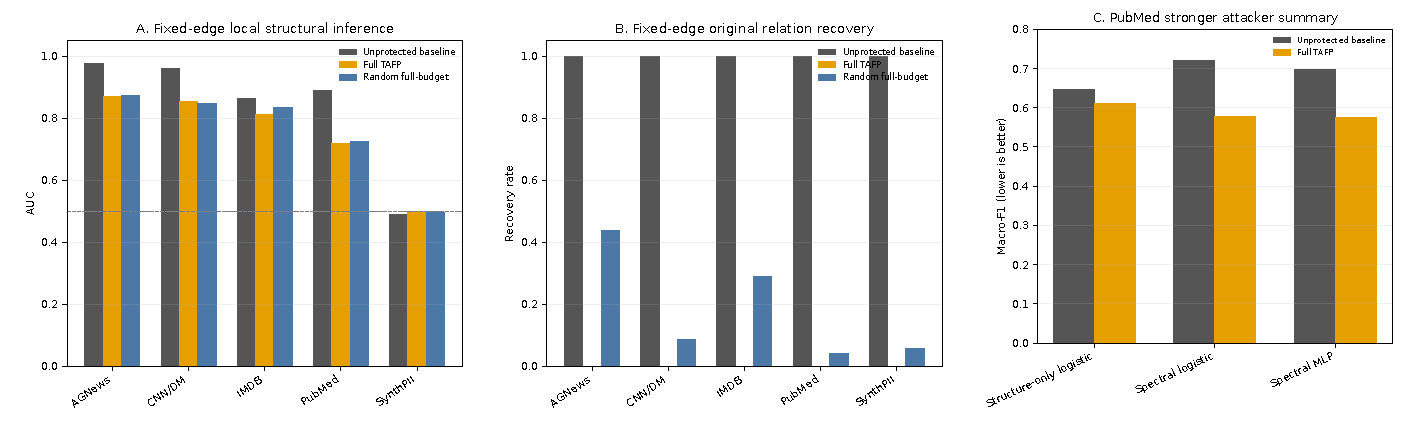
\includegraphics[width=\textwidth]{Figure_06.pdf}
\caption{Attack-specific relation-inference evidence. Panel A reports fixed-edge local structural AUC across the five evaluated datasets; the dashed line marks chance-level discrimination. Panel B reports direct recovery of the original relation label after deterministic sanitization for sensitive target edges. Panel C reports the PubMed stronger-attacker summary using only directly reported values: the structure-only logistic attack from Table 5 and the spectral logistic and spectral MLP attackers from Section 6.3. For Panel C, lower Macro-F1 indicates lower relation-inference success. Random full-budget is not shown for the spectral attackers because those exact values are not directly tabulated in the manuscript.}
\label{fig:6}
\end{figure}
\subsection{Structural and Retrieval-Grounded Utility}
Across the five datasets, full TAFP-GraphRAG retained a substantial fraction of the edge support used by the fixed retrieval paths. Mean query-support edge retention ranged from 0.81359 to 0.86568, while the complete original path was preserved for 0.67237--0.75662 of queries (Table~\ref{tab:7}). Endpoint reachability remained 1.0 in every dataset under the full configuration. Reachability within the original hop budget ranged from 0.71111 to 0.86697, and reachability within three hops ranged from 0.75796 to 0.99246. The strongest three-hop preservation was observed on PubMed, whereas SynthPII showed the largest structural displacement under the same protocol.

The relevant-subgraph results showed the same distinction between preserving retrieval access and preserving exact local structure. Under full protection, relevant-node recall ranged from 0.72295 to 0.86591 and relevant-edge recall from 0.66491 to 0.73790. The corresponding Jaccard ranges were 0.59406--0.78626 for nodes and 0.50825--0.61775 for edges (Table~\ref{tab:8}). Thus, most originally relevant nodes and a majority of originally relevant edges remained available, but the transformed contexts were not identical to the original induced subgraphs.

The matched \nolinkurl{random_full_budget} control produced broadly similar structural utility. Sixteen of the 20 paired path comparisons and 19 of the 20 paired subgraph comparisons were non-significant after Holm correction (Supplementary Tables S8--S9). The four significant path differences all occurred on IMDB and favored the matched random control. The only significant subgraph difference was SynthPII relevant-node recall, which was also lower under full protection. These results do not establish a general structural-utility advantage for sensitivity-guided selection over the matched random full-budget condition.

The deletion-only control retained more of the original structure on most measures. Compared with random edge dropout, full protection had lower means in 19 of 20 path comparisons and all 20 subgraph comparisons; all of these paired comparisons were significant after Holm correction. This contrast should be interpreted by objective rather than by structural overlap alone: random edge dropout directly optimizes neither selective concealment of policy-designated relation semantics nor the degree-preserving behavior evaluated for the designated TAFP variants.

Overall, the fixed-query evaluation shows that TAFP-GraphRAG preserved endpoint access and retained substantial path and local-subgraph support while altering enough of the original graph to reduce exact structural overlap. These metrics quantify retrieval-grounded structural utility only; generated-answer utility and sensitive-relation disclosure are evaluated separately in the end-to-end relation-QA protocol.

Table~\ref{tab:7} directly reports endpoint reachability and reachability within the original and three-hop budgets for the fixed source--target pairs, while Supplementary Table S17 reports component-count and largest-component-ratio deviations for the matched 2K analysis. The protocol did not compute a global average shortest-path length, so no whole-graph path-length claim is made.

\begin{landscape}
\begingroup
\scriptsize
\setlength{\tabcolsep}{1.5pt}
\begin{longtable}{|L{0.07\linewidth}|L{0.15\linewidth}|C{0.13\linewidth}|C{0.12\linewidth}|C{0.12\linewidth}|C{0.14\linewidth}|C{0.13\linewidth}|}
\caption{Fixed-query path-level structural utility. Endpoint reachability applies to the predefined source-target pairs and is not a global graph-connectivity measure.}\label{tab:7}\\
\hline
\makecell[bc]{\fontsize{5.2}{5.8}\selectfont\bfseries Dataset} & \makecell[bc]{\fontsize{5.2}{5.8}\selectfont\bfseries Variant} & \makecell[bc]{\fontsize{5.2}{5.8}\selectfont\bfseries Query-support edge\\retention} & \makecell[bc]{\fontsize{5.2}{5.8}\selectfont\bfseries Exact path\\preservation} & \makecell[bc]{\fontsize{5.2}{5.8}\selectfont\bfseries Endpoint\\reachability} & \makecell[bc]{\fontsize{5.2}{5.8}\selectfont\bfseries Reachable within\\original hop} & \makecell[bc]{\fontsize{5.2}{5.8}\selectfont\bfseries Reachable within\\three hops} \\ \hline
\endfirsthead
\hline
\makecell[bc]{\fontsize{5.2}{5.8}\selectfont\bfseries Dataset} & \makecell[bc]{\fontsize{5.2}{5.8}\selectfont\bfseries Variant} & \makecell[bc]{\fontsize{5.2}{5.8}\selectfont\bfseries Query-support edge\\retention} & \makecell[bc]{\fontsize{5.2}{5.8}\selectfont\bfseries Exact path\\preservation} & \makecell[bc]{\fontsize{5.2}{5.8}\selectfont\bfseries Endpoint\\reachability} & \makecell[bc]{\fontsize{5.2}{5.8}\selectfont\bfseries Reachable within\\original hop} & \makecell[bc]{\fontsize{5.2}{5.8}\selectfont\bfseries Reachable within\\three hops} \\ \hline
\endhead
AGNews & baseline & 1.0000 $\pm$ 0.0000 & 1.0000 $\pm$ 0.0000 & 1.0000 $\pm$ 0.0000 & 1.0000 $\pm$ 0.0000 & 1.0000 $\pm$ 0.0000 \\ \hline
AGNews & full & 0.8657 $\pm$ 0.0244 & 0.7566 $\pm$ 0.0420 & 1.0000 $\pm$ 0.0000 & 0.8268 $\pm$ 0.0277 & 0.9320 $\pm$ 0.0145 \\ \hline
AGNews & \nolinkurl{random_edge_dropout} & 0.9231 $\pm$ 0.0123 & 0.8507 $\pm$ 0.0255 & 0.9974 $\pm$ 0.0048 & 0.8813 $\pm$ 0.0196 & 0.9441 $\pm$ 0.0117 \\ \hline
AGNews & \nolinkurl{random_full_budget} & 0.8578 $\pm$ 0.0222 & 0.7387 $\pm$ 0.0362 & 1.0000 $\pm$ 0.0000 & 0.8169 $\pm$ 0.0274 & 0.9303 $\pm$ 0.0139 \\ \hline
CNN\_DM & baseline & 1.0000 $\pm$ 0.0000 & 1.0000 $\pm$ 0.0000 & 1.0000 $\pm$ 0.0000 & 1.0000 $\pm$ 0.0000 & 1.0000 $\pm$ 0.0000 \\ \hline
CNN\_DM & full & 0.8308 $\pm$ 0.0144 & 0.7003 $\pm$ 0.0239 & 1.0000 $\pm$ 0.0000 & 0.7749 $\pm$ 0.0200 & 0.9028 $\pm$ 0.0132 \\ \hline
CNN\_DM & \nolinkurl{random_edge_dropout} & 0.9157 $\pm$ 0.0149 & 0.8400 $\pm$ 0.0276 & 0.9993 $\pm$ 0.0014 & 0.8671 $\pm$ 0.0262 & 0.9347 $\pm$ 0.0170 \\ \hline
CNN\_DM & \nolinkurl{random_full_budget} & 0.8258 $\pm$ 0.0186 & 0.6940 $\pm$ 0.0299 & 1.0000 $\pm$ 0.0000 & 0.7658 $\pm$ 0.0294 & 0.8966 $\pm$ 0.0190 \\ \hline
IMDB & baseline & 1.0000 $\pm$ 0.0000 & 1.0000 $\pm$ 0.0000 & 1.0000 $\pm$ 0.0000 & 1.0000 $\pm$ 0.0000 & 1.0000 $\pm$ 0.0000 \\ \hline
IMDB & full & 0.8358 $\pm$ 0.0223 & 0.7029 $\pm$ 0.0350 & 1.0000 $\pm$ 0.0000 & 0.7783 $\pm$ 0.0316 & 0.8950 $\pm$ 0.0172 \\ \hline
IMDB & \nolinkurl{random_edge_dropout} & 0.9218 $\pm$ 0.0204 & 0.8482 $\pm$ 0.0378 & 0.9963 $\pm$ 0.0070 & 0.8745 $\pm$ 0.0347 & 0.9251 $\pm$ 0.0252 \\ \hline
IMDB & \nolinkurl{random_full_budget} & 0.8532 $\pm$ 0.0252 & 0.7341 $\pm$ 0.0397 & 1.0000 $\pm$ 0.0000 & 0.8012 $\pm$ 0.0346 & 0.9080 $\pm$ 0.0225 \\ \hline
PubMed & baseline & 1.0000 $\pm$ 0.0000 & 1.0000 $\pm$ 0.0000 & 1.0000 $\pm$ 0.0000 & 1.0000 $\pm$ 0.0000 & 1.0000 $\pm$ 0.0000 \\ \hline
PubMed & full & 0.8317 $\pm$ 0.0221 & 0.7089 $\pm$ 0.0326 & 1.0000 $\pm$ 0.0000 & 0.8670 $\pm$ 0.0199 & 0.9925 $\pm$ 0.0051 \\ \hline
PubMed & \nolinkurl{random_edge_dropout} & 0.9198 $\pm$ 0.0141 & 0.8468 $\pm$ 0.0252 & 0.9991 $\pm$ 0.0014 & 0.9142 $\pm$ 0.0168 & 0.9808 $\pm$ 0.0071 \\ \hline
PubMed & \nolinkurl{random_full_budget} & 0.8316 $\pm$ 0.0184 & 0.7053 $\pm$ 0.0255 & 1.0000 $\pm$ 0.0000 & 0.8644 $\pm$ 0.0210 & 0.9913 $\pm$ 0.0065 \\ \hline
SynthPII & baseline & 1.0000 $\pm$ 0.0000 & 1.0000 $\pm$ 0.0000 & 1.0000 $\pm$ 0.0000 & 1.0000 $\pm$ 0.0000 & 1.0000 $\pm$ 0.0000 \\ \hline
SynthPII & full & 0.8136 $\pm$ 0.0185 & 0.6724 $\pm$ 0.0295 & 1.0000 $\pm$ 0.0000 & 0.7111 $\pm$ 0.0287 & 0.7580 $\pm$ 0.0204 \\ \hline
SynthPII & \nolinkurl{random_edge_dropout} & 0.9127 $\pm$ 0.0172 & 0.8384 $\pm$ 0.0277 & 0.9974 $\pm$ 0.0063 & 0.8485 $\pm$ 0.0278 & 0.8613 $\pm$ 0.0273 \\ \hline
SynthPII & \nolinkurl{random_full_budget} & 0.8250 $\pm$ 0.0218 & 0.6881 $\pm$ 0.0319 & 1.0000 $\pm$ 0.0000 & 0.7263 $\pm$ 0.0327 & 0.7685 $\pm$ 0.0292 \\ \hline
\end{longtable}
\endgroup
\end{landscape}
\begin{landscape}
\begingroup
\scriptsize
\setlength{\tabcolsep}{1.5pt}
\begin{longtable}{|L{0.08\linewidth}|L{0.17\linewidth}|C{0.15\linewidth}|C{0.15\linewidth}|C{0.15\linewidth}|C{0.15\linewidth}|}
\caption{Relevant-subgraph structural utility. Recall measures retention of original evidence, whereas Jaccard similarity additionally accounts for replacement structure.}\label{tab:8}\\
\hline
\makecell[bc]{\fontsize{5.2}{5.8}\selectfont\bfseries Dataset} & \makecell[bc]{\fontsize{5.2}{5.8}\selectfont\bfseries Variant} & \makecell[bc]{\fontsize{5.2}{5.8}\selectfont\bfseries Relevant-node\\recall} & \makecell[bc]{\fontsize{5.2}{5.8}\selectfont\bfseries Relevant-node\\Jaccard} & \makecell[bc]{\fontsize{5.2}{5.8}\selectfont\bfseries Relevant-edge\\recall} & \makecell[bc]{\fontsize{5.2}{5.8}\selectfont\bfseries Relevant-edge\\Jaccard} \\ \hline
\endfirsthead
\hline
\makecell[bc]{\fontsize{5.2}{5.8}\selectfont\bfseries Dataset} & \makecell[bc]{\fontsize{5.2}{5.8}\selectfont\bfseries Variant} & \makecell[bc]{\fontsize{5.2}{5.8}\selectfont\bfseries Relevant-node\\recall} & \makecell[bc]{\fontsize{5.2}{5.8}\selectfont\bfseries Relevant-node\\Jaccard} & \makecell[bc]{\fontsize{5.2}{5.8}\selectfont\bfseries Relevant-edge\\recall} & \makecell[bc]{\fontsize{5.2}{5.8}\selectfont\bfseries Relevant-edge\\Jaccard} \\ \hline
\endhead
AGNews & baseline & 1.0000 $\pm$ 0.0000 & 1.0000 $\pm$ 0.0000 & 1.0000 $\pm$ 0.0000 & 1.0000 $\pm$ 0.0000 \\ \hline
AGNews & full & 0.8424 $\pm$ 0.0240 & 0.7079 $\pm$ 0.0351 & 0.7379 $\pm$ 0.0253 & 0.6177 $\pm$ 0.0311 \\ \hline
AGNews & \nolinkurl{random_edge_dropout} & 0.8943 $\pm$ 0.0142 & 0.8943 $\pm$ 0.0142 & 0.8257 $\pm$ 0.0164 & 0.8257 $\pm$ 0.0164 \\ \hline
AGNews & \nolinkurl{random_full_budget} & 0.8340 $\pm$ 0.0246 & 0.6965 $\pm$ 0.0353 & 0.7290 $\pm$ 0.0279 & 0.6076 $\pm$ 0.0343 \\ \hline
CNN\_DM & baseline & 1.0000 $\pm$ 0.0000 & 1.0000 $\pm$ 0.0000 & 1.0000 $\pm$ 0.0000 & 1.0000 $\pm$ 0.0000 \\ \hline
CNN\_DM & full & 0.7890 $\pm$ 0.0144 & 0.6101 $\pm$ 0.0218 & 0.6724 $\pm$ 0.0156 & 0.5083 $\pm$ 0.0224 \\ \hline
CNN\_DM & \nolinkurl{random_edge_dropout} & 0.8830 $\pm$ 0.0216 & 0.8830 $\pm$ 0.0216 & 0.8170 $\pm$ 0.0224 & 0.8170 $\pm$ 0.0224 \\ \hline
CNN\_DM & \nolinkurl{random_full_budget} & 0.7845 $\pm$ 0.0207 & 0.6080 $\pm$ 0.0219 & 0.6635 $\pm$ 0.0217 & 0.5014 $\pm$ 0.0200 \\ \hline
IMDB & baseline & 1.0000 $\pm$ 0.0000 & 1.0000 $\pm$ 0.0000 & 1.0000 $\pm$ 0.0000 & 1.0000 $\pm$ 0.0000 \\ \hline
IMDB & full & 0.8003 $\pm$ 0.0280 & 0.6695 $\pm$ 0.0361 & 0.7105 $\pm$ 0.0299 & 0.5456 $\pm$ 0.0324 \\ \hline
IMDB & \nolinkurl{random_edge_dropout} & 0.8882 $\pm$ 0.0267 & 0.8882 $\pm$ 0.0267 & 0.8292 $\pm$ 0.0296 & 0.8292 $\pm$ 0.0296 \\ \hline
IMDB & \nolinkurl{random_full_budget} & 0.8142 $\pm$ 0.0312 & 0.6836 $\pm$ 0.0342 & 0.7234 $\pm$ 0.0331 & 0.5554 $\pm$ 0.0317 \\ \hline
PubMed & baseline & 1.0000 $\pm$ 0.0000 & 1.0000 $\pm$ 0.0000 & 1.0000 $\pm$ 0.0000 & 1.0000 $\pm$ 0.0000 \\ \hline
PubMed & full & 0.8659 $\pm$ 0.0199 & 0.7863 $\pm$ 0.0250 & 0.7219 $\pm$ 0.0211 & 0.6046 $\pm$ 0.0234 \\ \hline
PubMed & \nolinkurl{random_edge_dropout} & 0.9273 $\pm$ 0.0121 & 0.9273 $\pm$ 0.0121 & 0.8520 $\pm$ 0.0117 & 0.8520 $\pm$ 0.0117 \\ \hline
PubMed & \nolinkurl{random_full_budget} & 0.8659 $\pm$ 0.0161 & 0.7864 $\pm$ 0.0214 & 0.7204 $\pm$ 0.0168 & 0.6026 $\pm$ 0.0184 \\ \hline
SynthPII & baseline & 1.0000 $\pm$ 0.0000 & 1.0000 $\pm$ 0.0000 & 1.0000 $\pm$ 0.0000 & 1.0000 $\pm$ 0.0000 \\ \hline
SynthPII & full & 0.7230 $\pm$ 0.0253 & 0.5941 $\pm$ 0.0290 & 0.6649 $\pm$ 0.0255 & 0.5295 $\pm$ 0.0287 \\ \hline
SynthPII & \nolinkurl{random_edge_dropout} & 0.8601 $\pm$ 0.0188 & 0.8601 $\pm$ 0.0188 & 0.8274 $\pm$ 0.0188 & 0.8274 $\pm$ 0.0188 \\ \hline
SynthPII & \nolinkurl{random_full_budget} & 0.7350 $\pm$ 0.0187 & 0.6029 $\pm$ 0.0217 & 0.6765 $\pm$ 0.0191 & 0.5378 $\pm$ 0.0212 \\ \hline
\end{longtable}
\endgroup
\end{landscape}

\subsection{End-to-End Relation-Question-Answering Utility and Sensitive-Relation Disclosure}
The locked end-to-end evaluation completed all 43,080 planned model generations over 718 fixed queries, five datasets, 15 protection seeds, and four graph conditions. The execution audit reported no duplicate rows, no query-set drift, no determinism mismatches, and successful degree-preservation and 2K joint-degree checks (Supplementary Table S26). The primary analysis retained all 26 parse failures, corresponding to 0.06035\% of the generated records.

For non-sensitive relation questions, full TAFP-GraphRAG achieved a relation-token F1 of 0.640579, compared with 0.682930 for the unprotected baseline (Table~\ref{tab:9}). This corresponds to 93.8\% retention of baseline F1. The paired difference was -0.042351, with a 95\% interval of [-0.061646, -0.023055] and Holm-adjusted p = 0.000610. Retrieved-evidence recall also decreased from 0.976940 to 0.874470. In contrast, exact sequence match increased from 0.161537 to 0.184574, and exact faithfulness to the retrieved relation sequence increased from 0.181931 to 0.306207; both paired differences were significant after Holm correction. The result therefore reflects a bounded utility trade-off rather than lossless preservation.

For sensitive-relation questions, the disclosure rate decreased from 0.970000 under the baseline to 0.075600 under full TAFP-GraphRAG. The absolute reduction was 0.894400, corresponding to a 92.2\% relative reduction. Its 95\% interval was [0.890469, 0.898331], with Holm-adjusted p = 0.001863. Sensitive-token recall decreased from 0.932000 to 0.062978, while retrieved sensitive-evidence exposure decreased from 0.942000 to 0.049311.

The sensitivity-guided condition was also separated from both sensitivity-blind controls in the downstream task. Full TAFP-GraphRAG achieved relation-token F1 values 0.502270 and 0.501185 higher than \nolinkurl{random_full_budget} and 2K, respectively; both Holm-adjusted p values were 0.000183. At the same time, its sensitive-disclosure rate was 0.156933 lower than \nolinkurl{random_full_budget} and 0.169067 lower than 2K, with Holm-adjusted p = 0.001863 for both comparisons. These directions and adjusted significance results held for the two primary outcomes in each of the five datasets as well as in the overall analysis (Supplementary Table S25).

Performance remained dataset dependent. Under full protection, relation-token F1 ranged from 0.587031 to 0.706349, and sensitive-disclosure rate ranged from 0.000000 to 0.155333 (Supplementary Table S24). Disclosure was zero on PubMed and 0.011333 on SynthPII, but residual disclosure remained on CNN/DM, AGNews, and IMDB, reaching 0.155333 on IMDB. The parse-success-only sensitivity analysis left the principal full and baseline F1 and disclosure values unchanged.

Together with Section 6.4, these findings refine the empirical contribution. The method is not supported as a universal mechanism for maximizing structural overlap: the matched random full-budget control was often structurally similar. Under the predefined end-to-end relation-QA protocol, however, sensitivity-guided transformation preserved substantially more non-sensitive answering utility while disclosing fewer sensitive relations than both evaluated sensitivity-blind controls. This supports selective, task-grounded relation protection under the evaluated conditions; it does not establish formal privacy, complete concealment, raw-text privacy, or protection against all attackers.

\begin{landscape}
\begingroup
\scriptsize
\setlength{\tabcolsep}{1.5pt}
\begin{longtable}{|L{0.15\linewidth}|C{0.11\linewidth}|C{0.09\linewidth}|C{0.13\linewidth}|C{0.13\linewidth}|C{0.11\linewidth}|C{0.12\linewidth}|}
\caption{Retrieval-grounded end-to-end relation-QA results across five datasets. Values are means over 15 protection seeds. Higher values are better for relation-token F1, exact match, and retrieved-evidence recall; lower values are better for the three disclosure metrics. The locked protocol comprised 43,080 generations.}\label{tab:9}\\
\hline
\makecell[bc]{\fontsize{5.0}{5.5}\selectfont\bfseries Variant} & \makecell[bc]{\fontsize{5.0}{5.5}\selectfont\bfseries Relation-token\\F1} & \makecell[bc]{\fontsize{5.0}{5.5}\selectfont\bfseries Exact\\match} & \makecell[bc]{\fontsize{5.0}{5.5}\selectfont\bfseries Retrieved-evidence\\recall} & \makecell[bc]{\fontsize{5.0}{5.5}\selectfont\bfseries Sensitive-relation\\disclosure} & \makecell[bc]{\fontsize{5.0}{5.5}\selectfont\bfseries Sensitive-token\\recall} & \makecell[bc]{\fontsize{5.0}{5.5}\selectfont\bfseries Retrieved\\sensitive\\exposure} \\ \hline
\endfirsthead
\hline
\makecell[bc]{\fontsize{5.0}{5.5}\selectfont\bfseries Variant} & \makecell[bc]{\fontsize{5.0}{5.5}\selectfont\bfseries Relation-token\\F1} & \makecell[bc]{\fontsize{5.0}{5.5}\selectfont\bfseries Exact\\match} & \makecell[bc]{\fontsize{5.0}{5.5}\selectfont\bfseries Retrieved-evidence\\recall} & \makecell[bc]{\fontsize{5.0}{5.5}\selectfont\bfseries Sensitive-relation\\disclosure} & \makecell[bc]{\fontsize{5.0}{5.5}\selectfont\bfseries Sensitive-token\\recall} & \makecell[bc]{\fontsize{5.0}{5.5}\selectfont\bfseries Retrieved\\sensitive\\exposure} \\ \hline
\endhead
Unprotected baseline & 0.6829 & 0.1615 & 0.9769 & 0.9700 & 0.9320 & 0.9420 \\ \hline
Full TAFP & 0.6406 & 0.1846 & 0.8745 & 0.0756 & 0.0630 & 0.0493 \\ \hline
Random full-budget & 0.1383 & 0.0223 & 0.1596 & 0.2325 & 0.1735 & 0.1553 \\ \hline
2K & 0.1394 & 0.0238 & 0.1600 & 0.2447 & 0.1816 & 0.1643 \\ \hline
\end{longtable}
\endgroup
\end{landscape}
\begin{figure}[p]
\centering
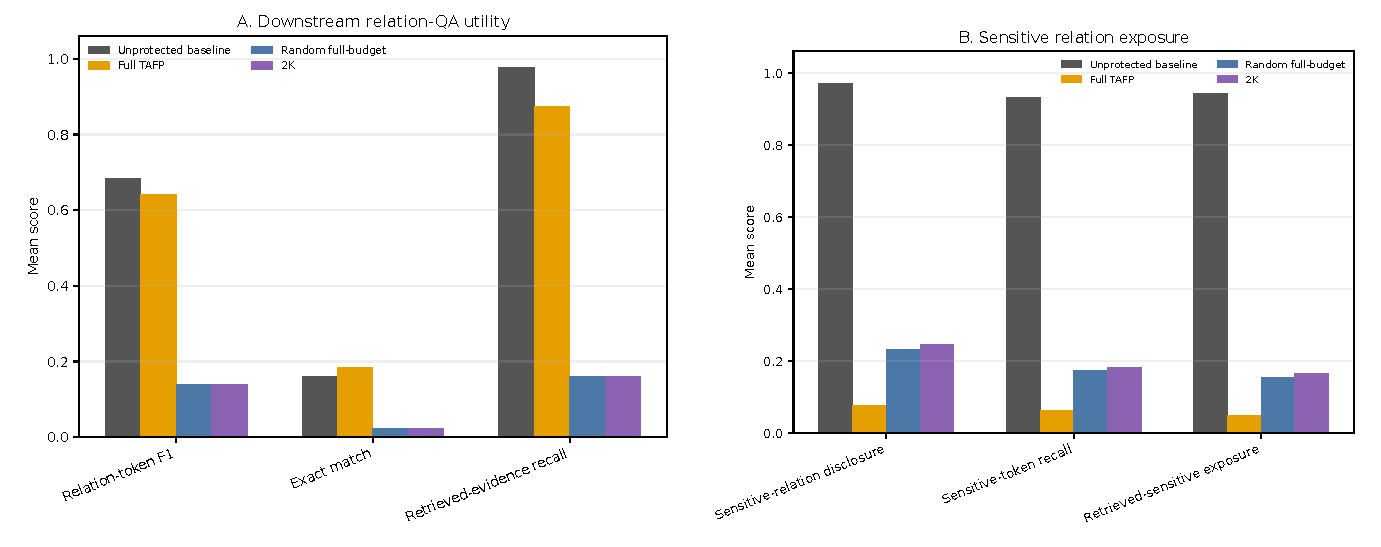
\includegraphics[width=\textwidth]{Figure_07.pdf}
\caption{End-to-end retrieval-grounded relation-QA utility and sensitive-relation exposure. Panel A reports relation-token F1, exact match, and retrieved-evidence recall for the unprotected baseline, Full TAFP, the random full-budget control, and the 2K baseline. Panel B reports sensitive-relation disclosure, sensitive-token recall, and retrieved-sensitive exposure, where lower values indicate lower downstream exposure. Values are aggregate results from the locked 43,080-generation evaluation protocol.}
\label{fig:7}
\end{figure}
\FloatBarrier
\section{Discussion}
\subsection{Policy Guidance Determines Where Information Loss Occurs}
The central empirical contribution is not perturbation alone, but policy-conditioned allocation of perturbation. Full TAFP-GraphRAG concealed 0.99993--1.00000 of policy-designated sensitive relation labels while retaining 0.89935--0.92193 of non-sensitive relation semantics. The perturbation-budget-matched random control retained nearly the same fraction of original edges, yet it concealed fewer sensitive labels and retained substantially less non-sensitive semantics. The minority-sensitive ablation reproduced the same concealment--retention profile from 5\% to 30\% sensitive-edge prevalence. These results isolate sensitivity guidance as the mechanism that determines which relation semantics are removed and which remain available.

This interpretation is narrower than a claim of universal optimization. At 5\% sensitive prevalence, the random relation-budget control retained more non-sensitive semantics, but it concealed only 0.0475 of sensitive labels, compared with 0.9996 under full protection. The relevant contribution is therefore selective information allocation under an explicit policy, not maximization of any single utility metric independently of the protection objective.

The comparative pattern depended on the evaluation objective. Policy guidance produced its largest gains when success required concealing designated labels while preserving the original semantics of non-sensitive edges, and it also separated from both sensitivity-blind controls in end-to-end relation QA. Matched random perturbation was more competitive for structural-overlap metrics and for several topology- or representation-based attackers under the same perturbation budget. Sensitive prevalence, label composition, and attacker observation surface therefore moderated the observed advantage; graph density and label entropy were not isolated as causal factors in the present design.

\subsection{Relation Privacy Must Be Evaluated Across Distinct Attack Surfaces}
The results show that relation-label concealment, policy-membership privacy, original-edge privacy, and representation-based relation inference are different security properties. Direct recovery of policy-designated sensitive relation labels was eliminated under the evaluated relation-only and full protocols. This did not remove evidence that an original edge had existed: hybrid edge-inference AUC remained high on several datasets. Topology-only, spectral, and released-view GCN-GAE attacks were also dataset dependent. PubMed showed significant reductions relative to the unprotected graph, but the matched random full-budget control was statistically competitive; SynthPII did not show a consistent reduction.

The marker audit identified an additional release-layer risk. The default PRIVATE\_RELATION marker and relation-label omission both revealed supplied-policy membership perfectly in the evaluated protocol. Coarse shared markers reduced that leakage only by sacrificing non-sensitive semantic retention. Consequently, a protected graph cannot be assessed solely by checking whether the original sensitive label is absent. The released schema, marker vocabulary, retained topology, and learned graph representations each define a separate observation surface and require separate measurements.

\subsection{Structural Invariants Constrain Transformation but Do Not Establish Privacy}
Exact per-node degree preservation was satisfied in every designated degree-preserving condition, and the 2K control additionally preserved the complete joint-degree distribution. These are strong and directly auditable structural invariants. They do not, however, imply relation privacy or semantic selectivity. The 2K control did not reproduce the concealment and non-sensitive retention achieved by the sensitivity-guided method, and identical degree constraints did not prevent residual topology- or representation-based inference.

The evidence therefore assigns a specific role to structural invariants. They bound how the graph changes and support compatibility and reproducibility, while the sensitivity policy determines where semantic protection is applied. Neither role is equivalent to a formal differential-privacy guarantee. TAFP-GraphRAG should accordingly be interpreted as an empirical, policy-conditioned protection mechanism with verified structural constraints, not as a substitute for differential privacy.

Exact degree preservation can also retain distinctive degree signatures that may act as quasi-identifiers or auxiliary inference features. The study therefore treats the invariant as a compatibility constraint rather than a privacy objective.

\subsection{Utility Conclusions Depend on the Evaluation Layer}
The structural evaluation showed substantial preservation of retrieval support: all evaluated endpoint pairs remained reachable, most path-support edges were retained, and most relevant nodes and edges remained available. Nevertheless, the matched random full-budget control was structurally similar on most path and subgraph comparisons, and random edge dropout preserved more exact original structure on most measures. These findings do not support a general claim that sensitivity guidance maximizes structural overlap.

The end-to-end relation-QA results provide a different and more task-grounded comparison. Full TAFP-GraphRAG retained 93.8\% of baseline non-sensitive relation-token F1 and reduced sensitive-relation disclosure by 92.2\% relative to the baseline. It also achieved higher non-sensitive relation-token F1 and lower sensitive disclosure than both evaluated sensitivity-blind controls in the overall analysis and in every dataset. At the same time, retrieval recall and relation-token F1 remained below the unprotected baseline, whereas exact sequence match and exact faithfulness increased. These metric directions show why utility must be characterized jointly rather than reduced to a single structural or generation score.

Taken together, the results support a precise downstream claim: sensitivity guidance did not generally preserve more graph structure than an equal-budget random transformation, but under the predefined relation-QA protocol it preserved substantially more task-relevant non-sensitive answering utility while disclosing fewer sensitive relations than the evaluated sensitivity-blind controls.

\subsection{Policy Quality and Release Design Are Operational Dependencies}
The policy-misclassification experiment showed that TAFP-GraphRAG faithfully executes the supplied policy but does not repair it. False negatives reduced concealment measured against the oracle policy, while false positives reduced oracle non-sensitive preservation. This separates transformation correctness from policy correctness. In deployment, sensitivity-policy validation, versioning, and error auditing are therefore part of the protection process rather than external administrative details.

Release design requires the same treatment. A marker that conceals the original relation label may still expose whether an edge was designated sensitive. Eliminating this policy-membership signal through broader cover labels produced a direct semantic-utility cost in the evaluated settings. Operational use therefore requires an explicit decision about which disclosure object is protected: the original relation value, the fact of policy designation, the existence of an original edge, or some combination of these.

No evaluated shared-cover setting was universally optimal. Applying the cover to all non-sensitive relations reduced policy-membership AUC to chance but eliminated measured non-sensitive semantic retention, whereas partial covers produced intermediate leakage and utility.

\subsection{Implications for Security-Oriented GraphRAG Deployment}
The findings support an offline governance pattern in which policy selection, graph transformation, invariant checks, attack-specific evaluation, and hash-traceable audit records are completed before the protected graph is used for retrieval. This design is practically relevant because it exposes residual risks rather than treating the transformation name as evidence of privacy. It also allows deployment decisions to be conditioned on the actual threat model and on acceptable trade-offs between non-sensitive utility and the disclosure objects being protected.

Within the evaluated scope, TAFP-GraphRAG contributes a reproducible method for selective relation protection that combines sensitivity-aware semantic transformation, designated structural invariants, and attack-specific privacy--utility evaluation. Its strongest evidence concerns selective relation-semantic protection and downstream relation-QA behavior. Attack resistance remains dataset and adversary dependent, and the framework does not establish formal privacy, complete anonymization, raw-text privacy, or protection against adaptive multi-turn reconstruction.

\section{Limitations and Scope Boundaries}
The evidence supports selective protection of policy-designated relation semantics under the evaluated protocols, but it does not establish universal or formal privacy. TAFP-GraphRAG does not provide differential privacy or local differential privacy, and the reported structural invariants must not be interpreted as equivalent guarantees. The framework also does not address raw-text confidentiality, document-membership privacy, or complete anonymization.

Attack resistance was dataset and attacker dependent. Direct recovery of designated sensitive relation labels was eliminated in the evaluated relation-level protocols, but residual inference remained through other observation surfaces. Original-edge existence could remain inferable, and the strongest released-view GCN-GAE stress test retained non-trivial predictive performance on PubMed. In several attack settings, the matched \nolinkurl{random_full_budget} control was statistically competitive. The evaluated attacks therefore bound the demonstrated protection; they do not exhaust adaptive, coordinated, or future adversaries.

The attack coverage was not uniform across all datasets. The structure-only, spectral, and released-view GCN-GAE evaluations were conducted on PubMed and SynthPII, whereas the fixed-edge, semantic-selectivity, marker-leakage, policy-misclassification, structural-utility, and end-to-end protocols covered five datasets. The reported attack conclusions should therefore remain tied to their corresponding datasets and observation models.

The sensitivity policies derived for the public datasets are experimental proxy policies rather than validated enterprise confidentiality labels. The policy-misclassification results show that the transformation executes the supplied policy but does not correct it. False negatives can leave oracle-sensitive relations insufficiently protected, and false positives can remove non-sensitive semantics unnecessarily. Real deployments therefore require domain-specific policy construction, validation, version control, and error auditing before transformation.

The default protected marker did not conceal whether an edge belonged to the supplied sensitive-policy set. Shared cover labels reduced this policy-membership signal only with a measurable reduction in non-sensitive semantic retention. Consequently, the present framework does not simultaneously optimize original-label concealment, policy-membership concealment, edge-existence privacy, and semantic utility. Deployment must specify which disclosure objects are in scope.

Deployments should restrict released edge attributes through an explicit allowlist. This recommendation defines a deployment boundary and was not separately evaluated in the present experiments.

Utility preservation was substantial but not lossless. Full protection reduced non-sensitive relation-token F1 and retrieved-evidence recall relative to the unprotected baseline, even though it improved exact sequence match and exact faithfulness and outperformed both evaluated sensitivity-blind controls on the primary downstream outcomes. Structural overlap also was not generally higher than under the matched random full-budget control. The results therefore support a task-conditioned privacy--utility trade-off, not universal utility preservation.

The end-to-end findings are bounded to the locked model, fixed query set, datasets, graph-construction rules, sensitivity policies, and four evaluated graph conditions. The study did not evaluate adaptive multi-turn reconstruction, collusion across releases, continual graph updates, cross-domain enterprise deployment, or long-term policy drift. These extensions are important future evaluation directions, but their outcomes cannot be inferred from the present evidence.

Computational evidence is limited to apply\_variant runtime and the controlled 2K telemetry on the five evaluated graphs. Peak memory, proposal-level attempt counts, proposal-acceptance ratios, and empirical scaling beyond these graph sizes were not instrumented. The study therefore makes no claim about production throughput or asymptotic scalability.

\section{Conclusion}
This study introduced TAFP-GraphRAG as an empirical, policy-conditioned framework for protecting sensitive relation semantics in GraphRAG while preserving explicitly defined structural invariants and maintaining auditable transformation records. Across five datasets, the full configuration concealed 0.99993--1.00000 of policy-designated sensitive relation labels, retained 0.89935--0.92193 of non-sensitive relation semantics, and preserved the exact degree of every node in the designated degree-preserving conditions. Equal-budget random and 2K-constrained controls did not reproduce this semantic selectivity, showing that the observed protection profile depended on sensitivity-guided allocation rather than perturbation volume or degree constraints alone.

The attack evaluation also established the boundaries of this contribution. Direct recovery of designated sensitive relation labels was eliminated in the evaluated relation-level protocols, but original-edge existence and representation-based relation inference could remain possible. Attack reductions were dataset and attacker dependent, the matched random full-budget control was competitive in several attack settings, and the default protected marker revealed supplied-policy membership. These findings support attack-specific evaluation of protected GraphRAG releases rather than a single undifferentiated privacy score.

Utility results were likewise evaluation-layer dependent. Full TAFP-GraphRAG preserved substantial path and local-subgraph support but did not generally exceed the matched random full-budget control in structural overlap. However, under the predefined retrieval-grounded structured relation-sequence question-answering protocol with deterministic decoding, it retained 93.8\% of baseline non-sensitive relation-token F1 and reduced sensitive-relation disclosure by 92.2\% relative to the unprotected baseline. It also achieved higher non-sensitive relation-token F1 and lower sensitive disclosure than both evaluated sensitivity-blind controls overall and in every dataset.

The resulting contribution is therefore precise: under the evaluated policies, datasets, models, and threat models, TAFP-GraphRAG provides reproducible selective protection of relation semantics with exact degree preservation in designated variants and task-grounded privacy--utility benefits. It does not provide differential privacy, complete anonymization, raw-text privacy, edge privacy, topology privacy, or universal attack resistance. Future work should evaluate alternative release markers, validated domain policies, adaptive and cross-release attacks, continual graph updates, and real enterprise deployments without extending the present evidence beyond its verified scope.

\section*{Supplementary Materials}
The supplementary materials provide detailed evidence supporting the main findings, including variant-level integrity audits, conditional relation-recovery results, feature-ablation analyses, fixed-edge and multi-split attack details, path- and subgraph-level paired tests, semantic-selectivity comparisons, sensitive-relation schema documentation (Tables S1--S18), sensitivity-flag leakage and cover-set coarsening (Table S20), sensitivity-policy misclassification robustness (Table S21), spectral embedding-based relation-inference summaries and paired tests (Tables S22--S23), dataset-level end-to-end relation-QA results (Table S24), paired seed-level end-to-end comparisons (Table S25), the parse-failure and execution audit (Table S26), the minority-sensitive policy ablation (Table S27), and the released-view GCN-GAE summary and paired tests (Tables S28--S29). Parameter-sensitivity protocols are described in Section 5.2 and their verified evidence is retained in the supplementary and immutable experiment archives. Distributed evidence tables and audit records are linked through hash-verified manifests. A claim-to-test evidence map linking the principal manuscript claims to their primary outcomes, comparators, experimental scopes, inferential units, multiplicity procedures, and evidence locations is provided as a separate supplementary index.

\section*{CRediT authorship contribution statement}
Y{\i}lmaz Vural: Conceptualization, Methodology, Software, Validation, Formal analysis, Investigation, Resources, Data curation, Writing -- original draft, Writing -- review and editing, Visualization, Project administration.

\section*{Funding}
This research did not receive any specific grant from funding agencies in the public, commercial, or not-for-profit sectors.

\section*{Declaration of competing interest}
The author declares that there are no known competing financial interests or personal relationships that could have appeared to influence the work reported in this paper.

\section*{Ethics statement}
This study used publicly available benchmark datasets and synthetically generated data. It did not involve human participants, identifiable private human-subject data, clinical intervention, or animal subjects. Institutional review board approval and informed consent were therefore not applicable.

\section*{Data availability}
The study used publicly available benchmark datasets subject to their respective licenses and a synthetic dataset generated for this research. The processed experimental artifacts and hash-verified evidence archives are maintained in private storage during peer review. Relevant artifacts can be made available to the editor and reviewers upon reasonable request, subject to applicable dataset licenses, repository-access controls, and platform restrictions.

\section*{Code availability}
The implementation, evaluation scripts, configuration records, and verified evidence archives are maintained in a private version-controlled repository. Reviewer access can be provided upon reasonable request during peer review. A public archival release may be prepared following acceptance, subject to licensing, security, and repository-governance requirements.

\section*{AI-assisted figure declaration}
The scientific figures in this manuscript were not generated using generative AI. They were produced programmatically from verified source data and documented scientific specifications using TikZ and Matplotlib. All figure contents, labels, numerical values, and layouts were reviewed by the author.

\section*{Declaration of generative AI and AI-assisted technologies in the manuscript preparation process}
During the preparation of this work, the author used OpenAI ChatGPT to support language refinement, document organization, consistency checking, and formatting review. The tool was not treated as an author and did not independently determine the scientific claims, experimental design, results, or conclusions. The author reviewed and edited all AI-assisted material and takes full responsibility for the content of the article.

\section*{Acknowledgments}
The author acknowledges the computing environments used to execute and validate the experiments.

\FloatBarrier
\bibliographystyle{elsarticle-num}
\bibliography{references}
\end{document}
